%\begin{savequote}[8cm]
%Alles Gescheite ist schon gedacht worden.\\
%Man muss nur versuchen, es noch einmal zu denken.

%All intelligent thoughts have already been thought;\\
%what is necessary is only to try to think them again.
 % \qauthor{--- Johann Wolfgang von Goethe \cite{von_goethe_wilhelm_1829}}
%\end{savequote}

\chapter{\label{ch-experiment}Measuring the TMPTA principal Hugoniot}

\minitoc

\section{Introduction}

The previous chapters have discussed the excitement and potential advantages of wetted-foam ICF capsules, and explored the fusion performance that may be achieved using them. Foams are also exciting for a range of other fusion-relevant applications: laser beam smoothing and imprint mitigation \cite{Depierreux2009, Hu2018} (where the foam is used to spread energy from an incoming laser beam laterally, reducing the imprint issues associated with direct-drive), adiabat shaping \cite{Craxton2015, Bodner1998, Collins2005} (where the adiabat can be shaped so that the outside of the shell is higher adiabat - and thus less susceptible to instability growth - while the inner fuel is kept on a lower adiabat and can thus be better compressed), increasing absorption of Nd-laser light \cite{Skupsky2004} (as the laser can propogate further into the material, due to regions where it is underdense, compared to a uniform material), and increasing conversion from laser light into X-rays \cite{Shang2016}. As a result foams are of significant research interest; with particular interest on the topics of homogenisation (how the inhomogenous foam transitions over time to a homogeneous plasma) and the impact of micro-structure on foam compression \cite{Hazak1998, Cipriani2021, Cipriani2018a, Colvin2013}.

Despite all this research interest, and the excitement surrounding wetted-foam ICF capsules, the equation of state of foam materials is poorly characterised. The EOS of wetted-foam capsules was discussed in Section \ref{sec:MixedEOS}, where the lack of wetted-foam tables was discussed and the need for further investigation of this material highlighted. This is not a unique problem to wetted-foams however; foam materials generally are described in simulations simply as a low-density version of the homogeneous material on which they are based. This does not account for the foam structure on inhomogeneity, and previous experiments have shown such an approach can be inaccurate \cite{Nicolai2012}. This suggests that even mixed-EOS tables for wetted-foams may be a poor description, and also suggests a potential source of inaccuracy for the `hydrodynamic equivalent capsules' where dry foam is used.

This chapter presents an experiment designed to help study this problem through studying the shock compression of TMPTA plastic foam at 260~\unit{\milli\gram\per\centi\meter\cubed}, to obtain principal Hugoniot data for this foam that existing and future EOS tables can be compared against. This is a comparable material and density to that used in the hydrodynamic equivalent capsules, making them of direct relevance to these designs (and of interest more broadly to those studying foams more generally). The experiment was performed using the VULCAN kJ-class Nd:glass laser at the UKRI-STFC Rutherford Appleton Laboratory. First, an overview of the experiment is provided, and the different techniques and diagnostics used within the experiment are described. Then the preparation work performed before the experiment will be discussed. Finally, the challenges faced during the experiment itself will be considered, along with the changes made from the initial plan to overcome these issues. The analysis, results and interpretation will be considered in the subsequent chapter.

%Foams are a topic of interest for a variety of reasons. Their relevance to this thesis is obvious: their role in the wetted-foam capsules discussed extensively in previous chapters, and in the hydrodynamic-equivalent capsules proposed in Chapter \ref{ch-FurtherSims}. However, they also have potential application in laser beam smoothing and imprint mitigation \cite{Depierreux2009, Hu2018} (where the foam is used to spread energy from an incoming laser beam laterally, reducing the imprint issues associated with direct-drive), adiabat shaping \cite{Craxton2015, Bodner1998, Collins2005} (where the adiabat can be shaped so that the outside of the shell is higher adiabat - and thus less susceptible to instability growth - while the inner fuel is kept on a lower adiabat and can thus be better compressed), increasing absorption of Nd-laser light \cite{Skupsky2004} (as the laser can propogate further into the material, due to regions where it is underdense, compared to a uniform material), and increasing conversion from laser light into X-rays \cite{Shang2016}. As a result foams are of significant research interest; with particular interest on the topics of homogenisation (how the inhomogenous foam transitions over time to a homogeneous plasma) and the impact of micro-structure on foam compression \cite{Hazak1998, Cipriani2021, Cipriani2018a, Colvin2013}.

%Of particular significance to this thesis is the issue of describing foams using equation of state models. The inhomogeneity of the material could potentially have significant effect on the foam EOS, with the voids within the structure requiring energy to close before more regular compression can begin. This process is not well described in simulations, were it is common to see foams described low-density versions of the homogeneous material upon which they are based (as was done in the simulations in earlier sections). However, previous experiments have shown that such an approach can be inaccurate \cite{Nicolai2012}. Inaccuracies in the equation of state have significant implications for for the accuracy of such simulations, which presents a potential source of of uncertainty in describing wetted-foam implosions.

%This problem motivated an experiment to investigate the equation of state - through principal Hugoniot measurements - of fusion-relevant TMPTA plastic foam, using the VULCAN kJ-class Nd:glass laser at the UKRI-STFC Rutherford Appleton Laboratory. This experiment is described in this chapter. First, an overview of the experiment is provided, and the different techniques and diagnostics used within the experiment are described. Then the preparation work performed before the experiment will be discussed. Finally, the challenges faced during the experiment itself will be considered, along with the changes made from the initial plan to overcome these issues. The analysis, results and interpretation will be considered in the subsequent chapter.

%This experiment was a large international collaboration between a number of institutions, but the work I present in this thesis was my own unless stated otherwise. I prepared the initial proposal for the experiment, which my supervisor submitted as PI. I then performed most of the preparation work before the experiment (which was supported with advice and some simulation work by some of my collaborators). I attended the experiment for the full run, and was the scientific lead throughout, supported by a large number of collaborators. At the start of the experiment these collaborators also served as `target-area operator', before I took on this role for the final three weeks. Finally, I performed the large majority of the analysis, again supported with advice, data and some simulation work by my collaborators.

\section{Experiment overview and diagnostics}

A mutli-layer target, containing a layer of TMPTA plastic foam at an initial density of 260~\unit{\milli\gram\per\centi\meter\cubed}, was shocked via irradiation from the Vulcan laser. The target was a sandwich design consisting of four layers: an $\sim$~40~\si[per-mode=symbol]{\micro\meter} CH ablator, followed by an $\sim$~3~\si[per-mode=symbol]{\micro\meter} gold layer, an $\sim$~40~\si[per-mode=symbol]{\micro\meter} $\alpha$-quartz reference layer, and then finally the $\sim$~40~\si[per-mode=symbol]{\micro\meter} TMPTA foam. A schematic of this target can be seen in Figure \ref{fig:target}. VULCAN was used to irradiate the CH layer, ablating material and driving a strong shock through the target. The gold layer prevented pre-heating of the quartz/foam, by absorbing any x-rays generated in the coronal plasma.

\begin{figure}
\centering
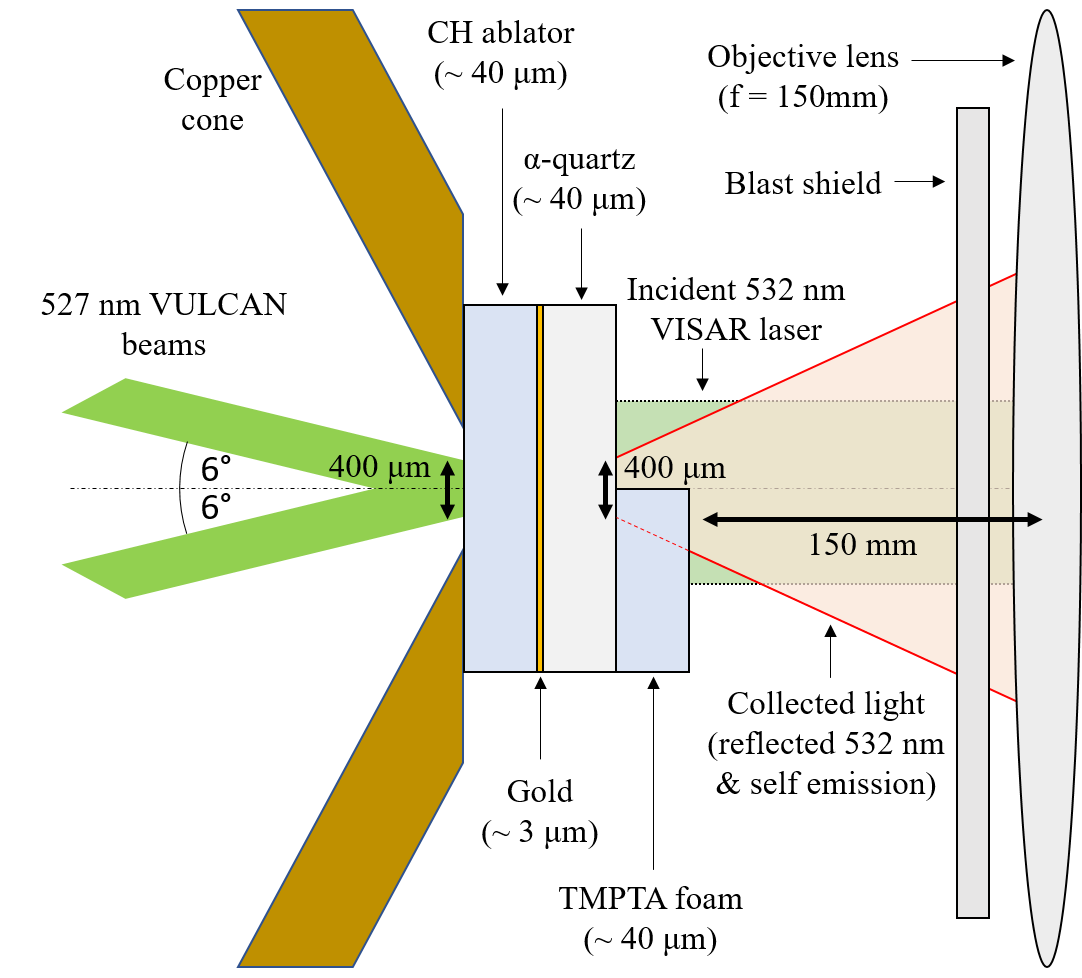
\includegraphics[width=0.45\textwidth]{figures/Experiment/TargetSchematic.png}% Here is how to import EPS art
\caption{\label{fig:target} Simple schematic showing the target and objective lens (top view, not to scale)}
\end{figure}

The six VULCAN long-pulse beams were overlapped spatially to produce a `top-hat' beam with a $\sim$~400~\unit{\micro\meter} diameter, generating a shock that was roughly uniform over this area. The pulse power profile was also a `top-hat', with a rise and fall time of $\sim$~200~\unit{\pico\second}. The target had a step in the rear side, so that the TMPTA foam only covered half of the quartz surface in the $\sim$~400~\unit{\micro\meter} shocked region. This meant that both quartz and foam were visible to the diagnostics, and is similar to targets used in previous experiments to investigate other materials \cite{Falk2014a, Falk2020}. The shock velocity in both layers was measured using VISAR, which was driven using a probe laser reflected off the rear surface of the target. The shock temperature of both layers was determined using streaked optical pyrometry (SOP).

The quartz layer in this experiment was used as a reference material for an impedance matching calculation. The shock velocity in both the quartz and the foam were measured in each shot and used to determine the foam shock state; the theory behind this process is described in Chapter \ref{ch-theory}, (Sections \ref{IMTheory} and \ref{IMTheoryMeasurements}). This defines a single shock state on the foam Hugoniot per shot. By performing a series of shots at different laser powers (and thus intensities), the Hugoniot curve could therefore be populated over a range of pressures.

\subsection{The VULCAN laser}

The VULCAN laser is based at the UKRI-STFC Rutherford Appleton Laboratory's Central Laser Facility. It is a 2.6 kJ Nd:glass laser with a fundamental frequency of 1053 \unit{\nano\meter}, with 8 beamlines (6 long-pulse, and 2 short-pulse) and two experimental areas providing different operational modes. At Target Area West, the 6 long-pulse beams are available alongside 2-short pulse beams. The long-pulse beams can each deliver energies ranging from 300 \unit{\joule} to 50 \unit{\joule}, dependent on pulse lengths ranging from 0.5 \unit{\nano\second} to 10 \unit{\nano\second}. These beams can be converted to second harmonic using KDP crystals (with some conversion losses) \cite{Ross1981}. The short-pulse beams can either both deliver 1 \unit{\pico\second} pulses, or offer a mixture of 1 \unit{\pico\second} and 10 1 \unit{\pico\second} pulses, with an intensity up to mid $10^{19}$ \unit{\watt\per\centi\meter\squared}. At Target Area Petawatt, a single short-pulse petawatt beam can provide intensities of up to $10^{21}$ \unit{\watt\per\centi\meter\squared} at shorter pulse times of $500$ \unit{\femto\second} (or lower powers and intensities for pulse times up to tens of \unit{\pico\second}), alongside a long-pulse beam line with the aforementioned properties.

Each beamline begins with a `seed' pulse, which is amplified to produce the main beam \cite{Ross1981}. For the long-pulse beams this seed is relatively high energy, and thus the preamplfication stage consists of a single rod amplifier \cite{Springate2010}. The pulse the enters the main amplification stage, where it is amplified by a series of further glass amplifiers. After each round of amplification, the beam diameter is increased; this reduces the intensity, which keeps it below the damage threshold of the laser glass. Rod amplifiers are used up to a diameter of 45 \unit{\milli\meter}, above which more efficient disk amplifiers are used \cite{Springate2010}. To produce short-pulse beams, chirped pulse amplification (CPA) \cite{Strickland1985} is used. Using this technique, a seed pulse is stretched temporally; this is then preamplified, and then amplified using the same conventional glass amplifiers\footnote{The petawatt beamline is preamplifed using optical parmetric CPA \cite{Ross1997,Hernandez-Gomez2006, Musgrave2015} instead due to the gain narrowing effect, as the short eventual pulse duration requires a minimum bandwidth \cite{Danson2004}.} up to the glass damage threshold, before being re-compressed in the target chamber to achieve a higher intensity short-pulse beam. 

%Producing short-pulse high intensity beams can be challenging, as above a threshold damage intensity the beam can no longer be amplified using conventional glass amplifiers. This issue was resolved by the invention of chirped pulse amplification (CPA) \cite{Strickland1985}. In this process, a relatively low power `seed' pulse with a short pulse length is `stretched' temporally, by chirping the beam so that the frequencies become separated out. The longer pulse can be amplified up to the damage threshold of conventional optics, before being compressed back to the original pulse length by reversing the chirp. This short-pulse now has an intensity significantly higher than that of the damage threshold.

%On VULCAN, CPA is used for the short-pulse beams. A short seed pulse is produced, stretched temporally, and then pre-amplified by a few rod amplifiers. The beam then undergoes the main amplification process described for the long-pulse beams, before being compressed in the target chamber.

%For the Petawatt beamline, a 120 \unit{\femto\second} initial pulse is stretched to 4.2 \unit{\nano\second} \cite{Hernandez-Gomez2006} and preamplified through mulitple rounds of optical parametric chirped pulse amplification (OPCPA) \cite{Musgrave2015}. OPCPA is a variation on CPA, where optical parametric amplification (OPA) is used - a process through which a powerful `pump' laser is used to amplify a weaker signal laser \cite{Ross1997}. OPA is used rather than glass amplifiers due to the gain narrowing effect; the eventual short pulse duration imposes a stringent minimum bandwidth requirement, and gain narrowing in glass amplifiers prevents this from being achieved \cite{Danson2004}. Using optical parametric amplification initially and then optimising the subsequent glass amplifiers to maximise this bandwidth enables this requirement to be satisfied. The pulse then undergoes amplification as described for the other beams.

%Finally, each beam is delivered to the target area. The short-pulse beams are compressed, reversing the effect of the chirp and resulting in a shorter and thus higher power laser pulse. All the beams also have a large diameter by this stage, and are focused down to a small spot to give a high intensity on target.

This experiment was conducted in Target Area West, and used only the six long-pulse beams. These were frequency doubled to second harmonic, and focused using custom phase plates into a single `top-hat' style laser spot with a diameter of 400 \unit{\micro\meter}. The same pulse was requested from each beam, coincident in time, to produce a single flat-topped laser pulse. This pulse time was varied throughout the experiment between 2 \unit{\nano\second} and 9 \unit{\nano\second}; this resulted in a range of pulse energies and intensities, thus driving shocks of a range of different strengths.

\subsection{VISAR}

VISAR (an acronym for `velocity interferometer system for any reflector') is a velocity interferometry technique, which allows the velocity of a moving surface to be detected \cite{Barker2000, Barker1972}. A probe laser is reflected from the surface to be measured, and the reflected light is passed into the interferometer (or `the VISAR'). The interferometer produces a fringe pattern, from which the velocity of the surface can be calculated. In this experiment, VISAR is used in this way to determine the shock velocity of the quartz (while also being used to identify breakout times, allowing the average foam shock velocity to be calculated).

A simple scehmatic of a VISAR is shown in Figure \ref{fig:VISAR_Schematic}. The interferometer consists of two legs. Leg `A' contains an etalon, and this serves to delay light passing through this leg by a time $\tau$ compared to the light passing through leg `B'. This means that a photon arriving from leg A at the recombination beamsplitter will have entered the VISAR a time $\tau$ earlier than a photon arriving at the same time from leg B. These photons will have therefore encountered the target at two different times, and (if the target is moving) two different positions. The total distance travelled by these two photons will therefore be a function of the surface velocity, which through the phase difference will be encoded into the resulting interference pattern.

\begin{figure}
\centering
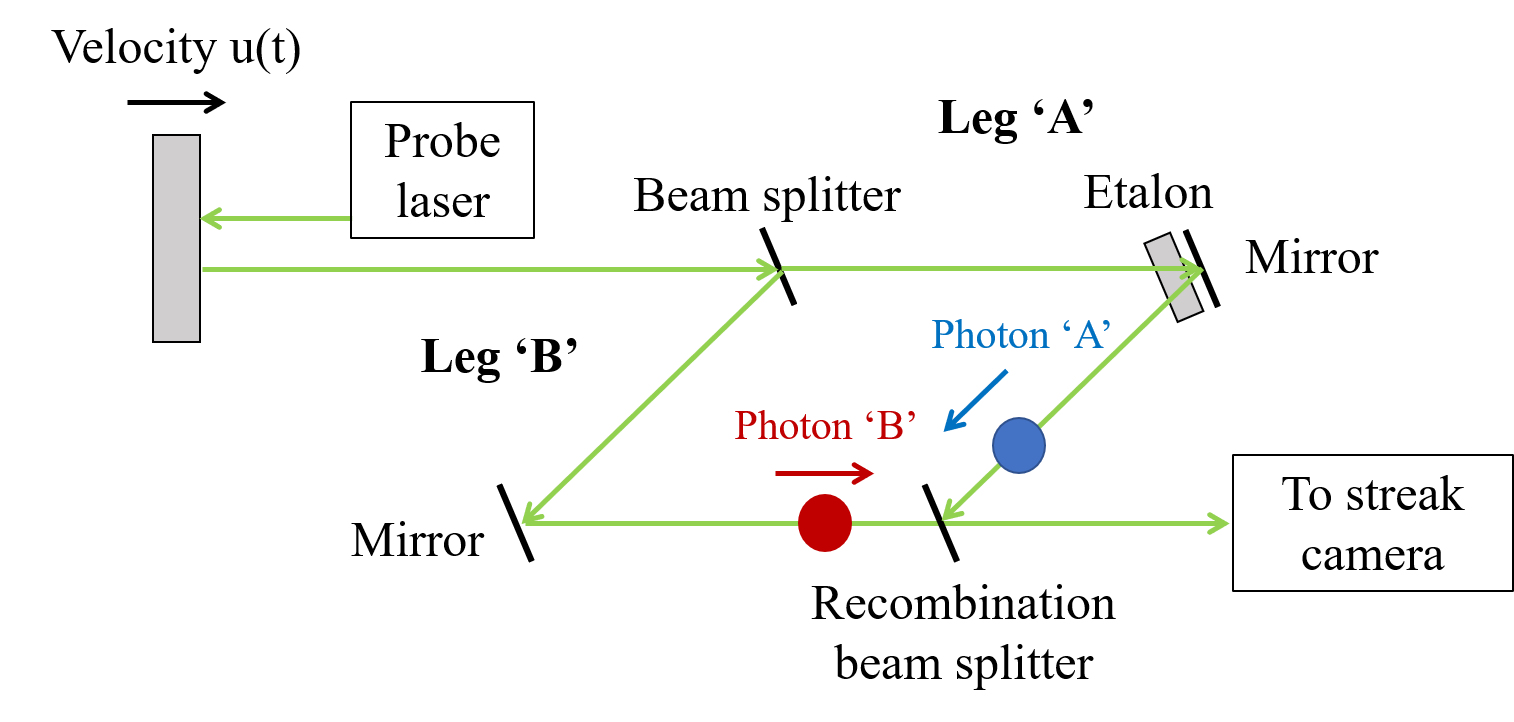
\includegraphics[width=0.6\textwidth]{figures/Experiment/VISARSchematic.png}% Here is how to import EPS art
\caption{\label{fig:VISAR_Schematic} Simple schematic of a VISAR. Photon `A' and photon 'B' travel down different legs to arrive at the recombination beam splitter at the same time and interfere with one another. These photons entered the VISAR (i.e. reached the first beam splitter) at different times; as the delay leg (leg 'A') takes an extra time $\tau$ to transit compared to leg 'B', photon 'A' must therefore have entered the VISAR a time $\tau$ earlier than photon 'B'.}
\end{figure}

Numerous mathematical descriptions of the VISAR exist. The one presented here is a simple explanation which considers the interference patter from an interferometry perspective, as presented originally in \cite{Barker1968} (and conceptually similar to the explanation given in \cite{Barker2000}). This derivation neglects the Doppler shift caused by the moving mirror, and instead simply considers the change in the mirror position in order to derive the correct result. Alternative derivations instead focus on the Doppler effect\footnote{The most simple form of this derivation is that presented in \cite{Barker1968}. Using the same variables defined in the main equation, the moving mirror introduces a doppler shift in the light of $\Delta \lambda (t) = - \frac{2 \lambda}{c} u(t)$. The length of the delay leg can be written in terms of multiples of the laser wavelength, $N \lambda = c \tau$. Differentiating this gives $\Delta N(t) = - \frac{c}{\lambda^2}\Delta \lambda (t)$. Substituting in the expression for $\Delta \lambda (t)$ then gives $u(t) = \frac{\lambda}{2\tau} \Delta N(t)$. The interference pattern is based on the difference in path length between the two legs, and thus the fringe shift is proportional to $\Delta N$ - leading to the same equation for the VPF as the main derivation.}, but then typically ignore the phase difference arising from the movement of the surface. Derivations based on this approach can be found in numerous sources \cite{Barker1968, Barker1972, Barker2000, Hammel2018}. More complete derivations are (such as those by Clifton \cite{Goosman1975a}, Goosman \cite{Goosman1975} and Bennett \cite{Bennett2016}) reconcile these two approaches, but are much more complicated.

Consider photons A and B in Figure \ref{fig:VISAR_Schematic}, which travel down the VISAR legs A and B respectively. Both arrive at the recombination beamsplitter at the same time. Photon A travelled down the delay leg, and thus took a time $\tau$ longer than photon B to travel through the VISAR - for them to arrive at the same time, it must therefore have entered the interferometer a time $\tau$ earlier.

Before entering the VISAR, both photons travel from the probe laser to the reflective surface, and then from the surface to the VISAR. For the photon `A', travelling at the earlier time, this distance can be denoted as $D$. If the surface is moving, then photon B travelling at a different time will encounter the surface in a slightly different position. It therefore travels a distance $D+2d$, where $d$ accounts for this small change (it is multiplied by two, accounting for the fact that the photon will travel this distance both to and from the surface). This distance d is given by \begin{equation} d = \int_{t_1}^{t_2} u(t') \cdot dt' = \int_{t_1}^{t_1 + \tau} u(t') \cdot dt',\end{equation} where $u(t')$ is the surface velocity as a function of time $t'$, $t_1$ is the earlier time at which photon A encounters the surface, and $t_2$ is the time at which photon B encounters it. The approximation $t_2 = t_1 + \tau$ has been made, which neglects the time taken for the photon to cover the distance d; this is reasonable, since the time $2d/c$ for the photon to travel this distance is typically much less than the time delay $\tau$ introduced by the etalon. The time $t_1 = t - T$ can be linked explicitly to the time at which the measurement is made at the streak camera $t$ by considering the time $T$ it takes the photon A to reach the streak camera; in this case, the distance $d = d(t)$ is itself a function of time.

The two photons therefore have a total path difference (when they interfere at the recombination beamsplitter) of $ \Delta x = 2d + \epsilon $, where $\epsilon$ is the (constant) additional path length introduced by the etalon. This leads to a phase difference of \begin{equation} \Delta\phi = k (2d + \epsilon),\end{equation} where $k = 2\pi / \lambda$ is the wave vector. Following the standard theory for interference between two waves \cite{Hecht2017}, the resulting intensity is given by  \begin{equation}I = I_1 + I_1 + 2\sqrt{I_1 I_2} \cos{\Delta \phi},\end{equation} where $I_1$ and $I_2$ are the intensity of the two waves in the different interferometer legs. As these are of equal intensity, $I_0 = 2 I_1 = 2 I_2$, this is simplified to \begin{equation} I = I_0 (1 + \cos{\Delta \phi}) = I_0 (1 + \cos{k (2d + \epsilon)}).\end{equation}

In this form, the intensity profile does not depend on spatial position (assuming that velocity is constant across the surface), and thus the interference `pattern' would be constant spatially. In order to produce spatial fringes, the recombination beamsplitter is rotated slightly to introduce a small linear phase ramp. This gives an intensity of \begin{equation} \label{eqn:VISAR eqn}I \propto  I_0 [1 + \cos(k (2d + \epsilon + x\sin(\theta) ))],\end{equation} where $x$ is the spatial position and $\theta$ is the (constant) angle of the beamsplitter, adding spatial dependence and resulting in a repeating pattern of fringes.

At this point, it is useful to consider two illustrative cases. First, consider the situation when the surface is stationary, or moving at a constant velocity $u_1$. In this case the distance $d(t)$ will be given by $d(t) = \tau u$, and will be constant. Equation \ref{eqn:VISAR eqn} will then feature no time dependence, and the fringe pattern will be constant as a function of time, described by 
\begin{equation} I(t_1) \propto I_0 [1 + \cos(\phi_1)] =  I_0 [1 + \cos(k (2\tau u_1 + \epsilon + x\sin(\theta)))].\end{equation}
Now, consider that the velocity of the surface changes to a new constant velocity $u_2$. This will result in a new fringe pattern described by \begin{equation}I(t_2) \propto I_0 [1 + \cos(\phi_2)] =  I_0 [1 + \cos(k (2\tau u_2 + \epsilon + x\sin(\theta)))] = I_0 [1 = cos(\phi_1 + 2k\tau \Delta u)] \end{equation}
representing a small fringe shift from the original pattern based on the difference in the two velocities $\Delta u = u_2 - u_1$. It is clear that there will be a single fringe shift when $2k\tau \Delta u = 2 m \pi$, where $m$ is any integer. The 'velocity per fringe', or VPF, is the velocity change that accompanies a full fringe shift, and is therefore defined as \begin{equation} VPF = \frac{\lambda}{2\tau}. \end{equation}

A small correction is applied to this equation, \begin{equation} VPF = \frac{\lambda}{2\tau (1 + \delta)}, \end{equation} to account for dispersion within the etalon $\delta$ \cite{Barker1974}. Further specific corrections can also be required depending on the precise experimental target configuration \cite{Barker1970, Celliers2004}.

This shift in fringes thus allows the velocity of the surface to calculated. The VISAR begins recording when the surface is stationary, and as the surface moves the total fringe shift is recorded. The VPF can then be used to calculate the surface velocity based on this fringe shift, allowing the velocity profile of the surface as a function of time to be determined. Analysis of VISAR data follows this principle, and a description of how this is performed in practice is provided in Appendix \ref{appdx: VISAR analysis}.

%\subsection{Old VISAR explanation}

%VISAR (or `Velocity Interferometer System For Any Reflector') is a velocity interferometry technique which allows the velocity of a moving surface to be measured. A probe laser is reflected from the measurement surface, and the reflected light captured and passed into the interferometer (often referred to as `the VISAR'). The resulting fringe pattern contains information about velocity changes at the surface. In this experiment, the VISAR is used to determine the shock velocity of both the quartz and the foam.

%A simple schematic of a VISAR is shown in figure. The reflected probe laser is split by a beamsplitter, and passes down two seperate legs, before being interfered at a recombination beamsplitter. An etalon is used so that the delay leg has a longer optical path, and thus a longer transmission time. This means that the photons interfering at the beamsplitter from the two different legs entered the interferometer at differnt times, and thus the interference is thus between the laser, and the laser released a short time previously.

%The effect of this is that the photons being interfered at the recombination beamsplitter entered the 

%This has a significant effect. As there is a difference in the transmission time through the two legs ($\tau$), two photons which arrive at the recombination beamsplitter entered the interferometer at different times. This means the interference is between the laser light, and the laser light a time $\tau$ previously. The resulting interference pattern thus is due to the changes in the phase of the beam over time. 

%These phase changes arise from the movement of the target, which is what enables velocity measurements using this technique. Consider the photon that arrives first. To reach the interferometer, the photon travelled from the laser to the measurement surface, and then back to the interferometer - a distance $D$. Now consider the second photon. In the time $\tau$, the surface has moved by a distance $d = \tau u$, where u is the average velocity of the surface over that time. The total distance the second photon travels is therefore $D+2d$ - a longer distance, which results in a phase shift (the factor 2 accounts for the fact that this distance must be covered twice. (A more rigorous analysis would include the fact that it would take some time to cover the distance d, but this is essentially negligible given that the the photon travels at the speed of light).

%The total path difference of the two beams at the recombination beamsplitter is therefore $\tau u + \delta$, where $\delta$ is the additional path length introduce by the delay etalon. This path difference results in a phase difference of $\phi = k (\tau u + \delta)$, where $k = 2\pi / \lambda$ is the wave vector. The resulting interference pattern varies according to the phase as $cos(\phi) = cos(k (\tau u + \delta)$. As described, and assuming no spatial variation in the reflector, the phase difference would be spatially constant. In order to produce a fringe pattern, the beamsplitter is rotated slightly to introduce a small linear phase ramp in the spatial position $x$, so that $\phi = k (\tau u + \delta + xsin\theta)$. This means that the image is now a fringe pattern.

%Consider the case where the surface is stationary or moving at a constant velocity, so that $u$ is a constant. In this case, the phase difference $\phi$ between the two signals is constant as a function of time, and thus the interference pattern is stationary - resulting in a static fringe pattern. However, consider the case where the surface velocity is changing, and thus $u$ varies. In this case, the phase will change by $k\tau \Delta u$, and thus the fringe pattern will also move. The pattern will repeat when $k\tau \Delta u = n\pi$ where n is an integer, and thus a full fringe change will occur when the change in velocity $\Delta u = \lambda /2 \tau$.

%In this way, the velocity of the surface can be determined. The experiment is begun with a stationary surface, and as the velocity changes the fringe pattern will be altered. The fringe shift F(t) is recorded, and can be converted into a velocity using this `Velocity per fringe', or VPF. This enables dynamic measurement of velocity vs time. The VPF needs an additional correction to account for dispersion, which leads to an actual VPF of \hl{equation}

\subsubsection{Etalon selection}

The etalon used in the VISAR determines the delay time $\tau$, and thus determines the VPF of the system. Using a thicker etalon results in a larger time delay and a lower velocity per fringe, giving increased velocity resolution. The value of $\tau$ also determines the time resoltion of the system; if a velocity change occurs in a time less than $\tau$, it will be recorded as a sudden discontinuity in the phase pattern.

Accurate determination of the velocity requires the fringe shift F(t) to be known. A discontinuity in the phase pattern prevents F(t) from being known with certainty, as the fringe pattern repeats if velocity increases by the VPF. A fractional phase shift could therefore correspond to a number of possible velocities, each seperated by integer multiples of the VPF. However, the ambiguity in velocity this causes can be resolved by introducing a second VISAR, using a different etalon. As long as the VPFs of the two etalons are not integer multiples, the different fractional phase shifts seen on the two VISARs will be unique to the a particular velocity, and thus the velocity can determined without ambiguity.

\subsubsection{VISAR design and operation}

A labelled diagram of the VISAR used in this experiment is displayed in Figure \ref{fig:Dan_VISAR}. This VISAR was developed and designed by Daniel Eakins. While the main components are the Mach-Zehnder interferometer, the overall device contains a series of optics to aid with alignment.

\begin{figure}
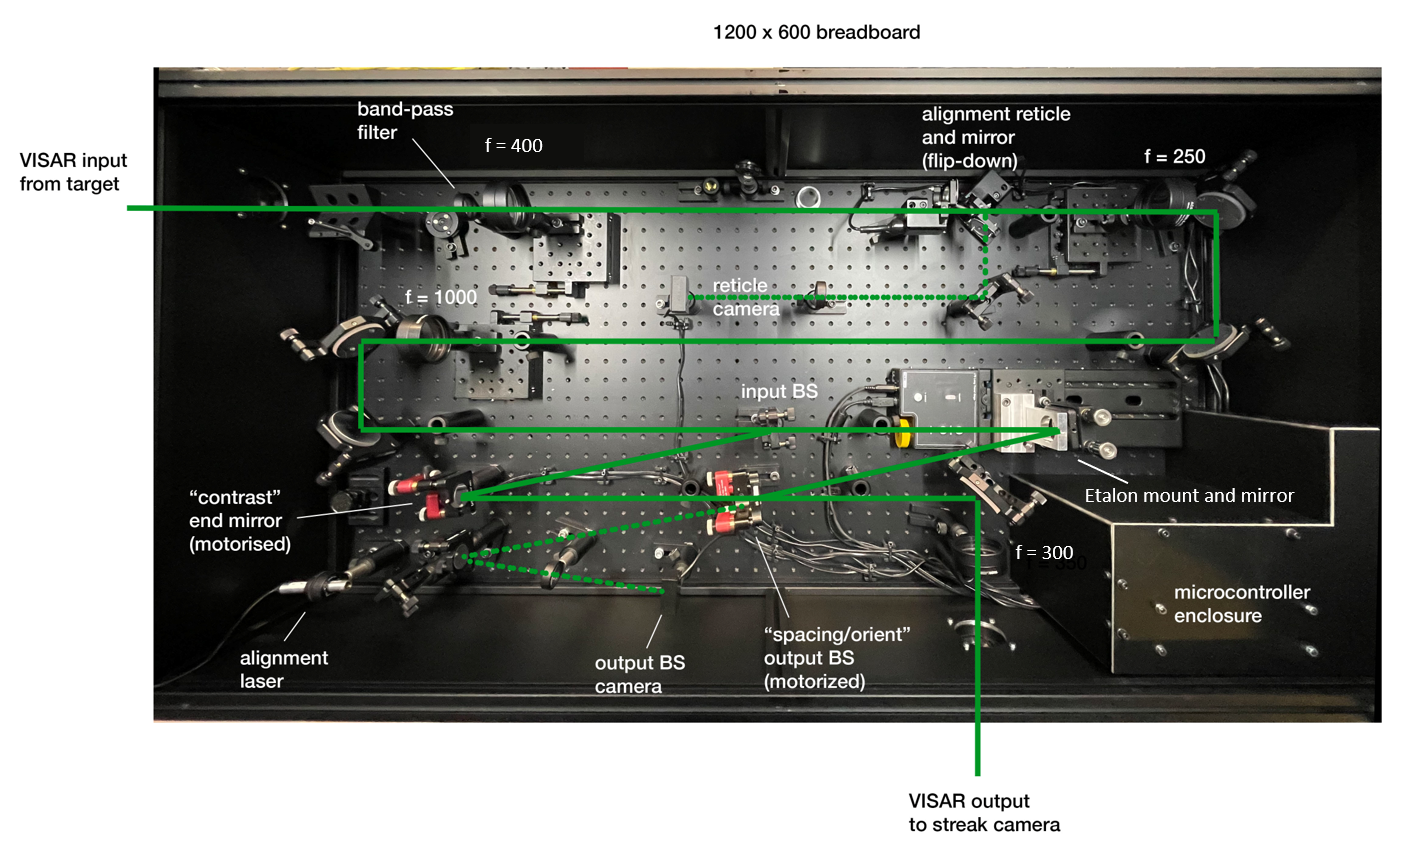
\includegraphics[width=1.0\textwidth]{figures/Experiment/Dan_VISAR.PNG}% Here is how to import EPS art
\caption{\label{fig:Dan_VISAR} The VISAR design used in this experiment (designed and developed by Daniel Eakins). The actual interferometer consists of the components between the input/output beamsplitters, while the other components are used for alignment and to ensure good image contrast. Image provided by Daniel Eakins, with minor changes to labels to reflect the lens setup used in our experiment. }
\end{figure}

The VISAR is internally aligned so that the first flip reticule is positioned in the center of the beampath. This can then easily be used to confirm that the external probe beam entering the VISAR is co-aligned with the system. However, it also serves another important purpose. The etalon and mirror in the delay leg are placed on a piezo-electric motor. As these components are aligned at an angle to the incoming beam, moving them will shift the position of the image. 

For VISAR operation it is required that these two images are aligned. To do this, the etalon is first removed from the delay leg. White light is injected into the VISAR, and the motorised stage on which the mirror and etalon mount sit in the delay leg moved until fringes appear. The white light is incoherent, and so fringes are only observed when the two legs have equal path length - this is sometimes referred to as the `null' or `white-light' position. The system is aligned so that the images are coincident for this seteup, which is confirmed by flipping the reticule into the beam and viewing the images at the output beamsplitter camera.

The etalon is then inserted. This introduces some refraction of the beam, and thus shifts the image. The etalon and mirror are thus translated on the motorised stage until the images are colinear again. This offset can be calculated\footnote{In practice, this offset is found experimentally, and this allows the angle $\theta_h$ to be calculated. This can then be used to accurately determine $\tau$ for the etalon.} by the formula \begin{equation} d = t \left(1 - \frac{\cos\theta_h}{n \cos(\sin^{-1}(\frac{\sin\theta_h}{n}))}\right), \end{equation} where $t$ and $n$ are the thickness and refractive index of the etalon, and $\theta_h$ is the angle of incidence between the laser and the VISAR components \cite{Bolme2013}. This results in a difference in path length which would prevent fringes from being observed with white length; however, the probe laser has a long coherence length, and thus this change is path length is not significant. Ensuring the images are coincident again ensures that the image has good spatial resolution, and also serves to increase fringe contrast - making the signal easier to detect. The time delay that the etalon introduces in a VISAR of this design can be calculated according to \begin{equation} \tau = \frac{2t (n - \frac{1}{n})}{c \cos(\sin^{-1}(\frac{\sin\theta_h}{n}))}, \end{equation} where $c$ is the speed of light \cite{Bolme2013}. 

The main benefit of a Mach-Zehnder design for the VISAR is that the use of two beamsplitters makes it possible to control the image alignment (and thus contrast) and the linear ramp/fringe spacing independently \cite{Celliers2004}. The `contrast mirror' is motorised, and can be adjusted to ensure the best possible overlap between images at the recombination beamsplitter, enabling contrast to be maximised. Independently, the recombination beamsplitter can be rotated to adjust the linear phase ramp, and thus change the number/spacing of the fringes (an important factor in analysing the resulting data). 

\subsubsection{Making shock velocity measurements with VISAR}

The previous descriptions describe how VISAR can be used to dynamically measure the velocity of a moving surface. Measuring shock velocity using VISAR introduces additional complexity, as the surface to be measured is a density interface within the target. To determine what exactly will be measured, it is necessary to consider which surface the VISAR will be reflected from, and it's properties.

The first way to measure shock velocity using VISAR is where the unshocked velocity is transparent to the probe beam, but the shocked material is reflective. In this case, the probe laser can propogate through the unshocked material, and reflect directly off the shock front; this shock front is the measurement surface, and the shock velocity can be measured directly \cite{Celliers2004}. This is the case for alpha-quartz (the reference used in this experiment), which for pressures above $\sim$ 100GPa becomes a conductive fluid with significant reflectivity at 532 \unit{\nano\meter} \cite{Hicks2006a}.

A different approach is required for opaque materials, such as the foam in this experiment. In this case the probe laser will reflect from the stationary front surface of the material; the VISAR will thus measure the velocity of the stationary surface, rather than the shock front. However, the VISAR can be used to detect changes to this surface. Fringes will be produced when the surface is intact, but will suddenly disappear when the surface is blown-out and stops reflecting - as occurs at shock breakout. By using steps in the material of known thickness and using the VISAR to identify the time at which the shock transits the steps, it is possible to calculate the average shock velocity through this region.

\subsubsection{VISAR application in this experiment}

In this experiment, the target has a step structure - so that half the rear surface is exposed quartz, and the other is foam. The spot is positioned over this step, so that half of the VISAR image corresponds to signal from the quartz and the other half from the foam. To illustrate this, some simulated VISAR data has been produced, and is displayed in Figure \ref{fig:VISARToy}. Figure \ref{fig:VISARToy} (a) shows simulated streak images of this VISAR data for two different etalon choices.

\begin{figure}
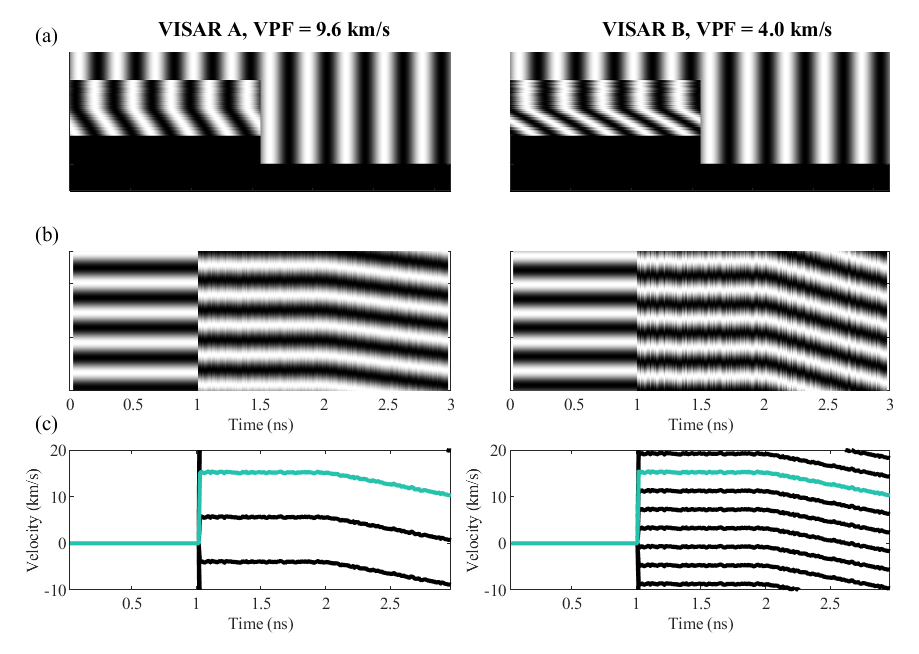
\includegraphics[width=1.0\textwidth]{figures/Experiment/VISARToy.eps}% Here is how to import EPS art
\caption{\label{fig:VISARToy} Simulated VISAR data for two different etalons. Row (a) shows the simulated streak image from each VISAR (where time increases with decreasing $y$ position, and the $x$ dimension represents different positions on the target. In row (b), portion of the data corresponding to the quartz has been selected, rotated, and a timescale added based on the simulated streak window. This has then undergone the filtering and phase unwrapping procedure described in the VISAR analysis section. In row (c), the resulting velocity traces for each VISAR are displayed. The discontinuity could correspond to any integer number of VPFs. However, using two VISARs with different etalons allows for unambiguous determination of the real velocity, since only one of these velocity traces is common to both VISARs (displayed in teal).}
\end{figure}

The underlying data for these simulated images has been chosen to best illustrate the key features/behaviours rather than representing realistic timings or shock profiles, and additional behaviours (such as changes in reflectivity) are neglected for simplicity. A 5 \unit{\nano\second} streak time/measurement window was chosen. For the first 1 \unit{\nano\second}, the shock is in the ablator/gold. The shock is in the quartz for the next 2 \unit{\nano\second}, and in the foam for a further 1 \unit{\nano\second} - breaking out of the rear of the target 1 \unit{\nano\second} before the end of the measurement window. The quartz shock velocity is constant at 15 \unit{\kilo\meter\per\second} for 1 \unit{\nano\second}, and then decays linearly to 10 \unit{\kilo\meter\per\second} over the next 1 \unit{\nano\second}. A small amount of Gaussian noise has been added to these velocities. These values are not representative of what is expected experimentally. The streak images have been created to match the real experimental measurements, with time increasing with decreasing $y$ position in the image, and the $x$ direction representing different points on the target. In this simple model the velocity is constant with position in the two regions; but as the VISAR has spatial resolution, a spatially varying velocity profile could also be measured.

The left half of each streak image in Figure \ref{fig:VISARToy} (a) corresponds to the quartz signal. Initially, the VISAR probe laser will pass through the quartz and reflect from the stationary gold layer. When the shock transits through from the gold to the quartz, the laser will begin to reflect from the shock front instead - leading to a sudden jump from a measured velocity of 0 to a measured velocity of $U_{s}^{quartz}$ (15 \unit{\kilo\meter\per\second} in this case). The sudden change in velocity results in a sudden fringe shift. These fringes are static in the new position while the shock velocity is constant, but as the shock velocity begins to decay the fringes are seen to shift smoothly as a function of time. The right side of the image shows the foam signal. The foam is opaque to the probe laser, which continues to reflect off the foam surface - this surface is stationary, and thus the fringe pattern is static.

When the shock breaks out from the quartz, the laser on the quartz side has no surface to reflect off and thus the fringes disappear. The laser on the fringe side continues to reflect off the stationary foam surface until the shock breaks out from this surface too, at which point fringe extinction again occurs. The $y$ position in the streak images can be converted to a time scale, based on the streak time, and thus the shock transit time through the quartz and the foam can be identified from these images, enabling calculation of the average shock velocity.

The quartz velocity can also be obtained as a function of time through VISAR analysis of these images. In Figure \ref{fig:VISARToy} (b), the quartz section of the image has been selected and rotated, and the time scale has been added. The VISAR analysis procedure \footnote{The code I used to do this was based on a VISAR analysis script provided by Daniel Eakins} described in Appendix \ref{appdx: VISAR analysis} was then applied to calculate the shock velocity profiles seen in Figure \ref{fig:VISARToy} (c). While the shock decay is larger than the 4 \unit{\kilo\meter\per\second} VPF of the second VISAR, the extended period this change occurs over means this can easily be resolved. However, the sudden change in shock velocity as the shock enters the quartz leads cannot be resolved, resulting in a fringe discontinuity. This could correspond to an infinite number of possible velocity jumps each seperated by an integer multiple of the VPF, as seen for each VISAR in Figure \ref{fig:VISARToy} (c). However, only the true velocity profile is common to both etalon choices \footnote{Mathematically, this leads to two simultaneous equations: $u = (m_1 + a) \cdot \textrm{VPF}_1$ and $u = (m_2 + b) \cdot \textrm{VPF}_2$, where $u$ is the true velocity, $m_1, m_2$ are the appropriate integer number of fringes missed in the discontinuity, and $a,b$ are the fractional fringe shifts measured in the two streak images. As both signals correspond to the same true velocity, the integers $m$ can be calculated and thus the true velocity determined.}. This is the teal profile displayed in Figure \ref{fig:VISARToy} (c). The shock velocity profile can thus be unambiguously determined.




%It is also necessary to include a translation offset in the delay leg, to account for the refractive index of the etalon. The etalon is placed at an angle to the beam, to avoid reflections from the etalon surfaces introducing interference; this however introduces refraction, which would shift the position of the beam at the recombination beamsplitter. To avoid this, the etalon and mirror in the delay leg are placed on a motorised stage. The etalon is removed, and the mirror translated to find the position corresponding to zero path difference. The etalon is then reinserted, and the mirror/etalon then repositioned until the image is coincident with the null position. this distance, $d = h(1 - 1/n)$ is then recorded. 

%The optical path difference between the delay and non-delay legs is $2(hn - h)$ (as the h thickness of etalon, with optical path $hn$, replaces a distance $h$ of air with a refractive index of 1. The factor 2 comes from the fact that the light passes through this etalon twice). Combining this and the translation offset gives a total path difference of $2h(n - 1/n)$, and thus an optical time delay of $\tau = 2h/c (n - 1/n)$.

%In any interferometer, the fringe frequency is the frequency difference (or beat frequency) of the two legs. In the velocity interferometer, this frequency difference is determined by the time dependent Doppler shift of the reflected light. The light being interfered is a reflection from the measurement surface at a time t1 and a time t1 + $\tau$. The Doppler shift of the reflected beam is dependent on the surface velocity, and thus the frequency difference between these two signals is also linked to the velocity. It is thus clear that the beat frequency will change as a function the velocity of the measurement surface, and thus the fringe pattern will change. However, the operation of the VISAR can be better illustrated by considering the path difference experienced by photons.

%The effect of the VISAR is to interfere photons that were reflected from the measurement surface at different times. At any given time, the photons being interfered at the recombination beamsplitter passed through the seperation beamsplitter at a time $\tau$ apart, and thus reflected from the measurement surface at different times. The measurement surface has a velocity $v(t)$, and thus a position $x(t)$. There will therefore be an additional path difference $\delta x$ between the two paths from the movement of the surface, introducing an additional optical time delay of $2h/c \delta x$.

%If the surface is stationary, then $\delta x$ is constant (zero) and the phase difference between the two legs is constant. The resulting interference pattern is thus unchanging as a function of time. If the surface is moving at a constant velocity, then $\delta x$ is also constant as a function of time. However, if there velocity of the surface is changing, then the phase change will also change, and the fringe pattern will move to reflect this. If the change is large and occurs much faster than the time resolution of the detector, this will result in discontinuities in the fringe pattern.

%The phase difference associated with this delay is given by $\Deltat\phi = kx = x/\Lambda$. As the fringe pattern is given by sin($\Deltat\phi$), one complete fringe corresponds to a phase difference of 2 pi.

\subsection{Streaked Optical Pyrometery} \label{SOP theory}

Streaked Optical Pyrometry enables the temperature of a body to be determined, based on it's thermal emission \cite{Zeldovich1966}. Emmitted light from the target is captured using measurement optics. This light is broadband, but can be filtered down to a narrow wavelength range using appropriate filters. This filtered emission is then recorded on a streak camera, which records the intensity vs time vs a spatial dimension.

%As described in \cite{Miller2007}, the intensity recorded on a streak camera at a given pixel is given by 
%\begin{equation} I = \frac{\Delta t}{G} \int {\Phi_S(\lambda) T_x(\lambda)SR(\lambda) d\lambda}, \end{equation} where $\Delta t$ is the dwell time (the amount of time over which signal is acquired for a given pixel), $G$ is the streak camera gain between photoelectrons and analogue to digital units, $T_x(\lambda)$ is the transmission between the object and the camera, and $SR(\lambda)$ is the SOP response function. $\Phi_S(\lambda)$ is the radiant power from the source. The power from the source that maps to a given pixel can be calculated as 
%\begin{equation} \Phi_S(\lambda) =  \int_{A_{pixel}}{ dA} \int_{\Omega_{lens}} { L_S(\lambda) d\Omega}, \end{equation}
%where $A_{pixel}$ is the source area represented per pixel, and $\Omega_{lens}$ is the solid angle captured by the imaging system. $L_S{\lamba}$ is the spectral radiance of the source. For a given optical setup of the streak camera (i.e. where the target is placed at the same location, the imaging system is not being changed, and the streak camera settings are constant), then these equations can be combined and simplified to 
%\begin{equation} I = \alpha \int {L_S(\lambda) T_x(\lambda)SR(\lambda) d\lambda}, \end{equation} where the proportionality constant $\alpha$ contains a number of variables relating to the specific setup used.

Following the derivation given in \cite{Miller2007}, the intensity recorded on a streak camera at a given pixel is given by \begin{equation} I = G \int {\Delta t} dt \int {\Phi_S(\lambda) T_x(\lambda)SR(\lambda) d\lambda}, \end{equation} where $G$ is a factor proportional to the streak camera gain, $\Delta t$ is the dwell time (the amount of time over which signal is acquired for a given pixel), $T_x(\lambda)$ is the transmission between the object and the camera, and $SR(\lambda)$ is the SOP response function. $\Phi_S(\lambda)$ is the radiant power from the source. The power from the source that maps to a given pixel can be calculated as 
\begin{equation} \Phi_S(\lambda) =  \int_{A_{pixel}}{ dA} \int_{\Omega_{lens}} { L_S(\lambda) d\Omega}, \end{equation}
where $A_{pixel}$ is the source area represented per pixel, and $\Omega_{lens}$ is the solid angle captured by the imaging system. $L_S (\lambda)$ is the spectral radiance of the source. For a given optical setup of the streak camera (i.e. where the target is placed at the same location, the imaging system is not being changed, and the streak camera settings are constant), then these equations can be combined and simplified to 
\begin{equation} I = \frac{B \Delta x W_s \Omega_{lens} G}{\eta M^2} \int {L_S(\lambda) T_x(\lambda)SR(\lambda) d\lambda}, \end{equation} where the variables outside the integral all relate to the specifics of the optical setup and streak camera settings ($B$ is the CCD binning, $W_s$ is the slit width, $\eta$ is the sweep rate, and $M$ is the magnification).

The source is then assumed to emit as a black body, such that the spectral radiance can be calculated using Planck's law, 
\begin{equation} L_S(\lambda) =  \frac{2hc^2}{\lambda^5} \frac{1}{[\exp(\frac{hc}{\lambda T}) - 1]}, \end{equation} where $T$ is the black-body temperature. The SOP signal is therefore given by 
\begin{equation} I = \frac{B \Delta x W_s \Omega_{lens} G}{\eta M^2} \int {\frac{2hc^2}{\lambda^5} \frac{<T_x(\lambda)SR(\lambda)>}{[\exp(\frac{hc}{\lambda T}) - 1]} d\lambda} \end{equation}
The incoming light is filtered down to a narrow wavelength band. The Fourier spectrum of the incoming light is therefore approximated as a delta function, at the central wavelength of this band. This simplifies the SOP signal to
\begin{equation} I = \frac{B \Delta x W_s \Omega_{lens} G}{\eta M^2} \frac{2hc^2}{\lambda_0^5} \frac{<T_x SR> }{ [\exp(\frac{hc}{\lambda T}) - 1]} , \end{equation}
This equation can then be rearranged to give an expression for temperature in terms of the measured intensity, 
\begin{equation} T = \frac{T_0}{\ln(1 + \frac{A}{I})}, \end{equation}
where $T_0 = \frac{hc}{\lambda_0}$ is a constant, and $A$ is a calibration constant,
\begin{equation} A = \frac{B \Delta x W_s \Omega_{lens} 2hc^2 <T_x SR> G}{\eta M^2 \lambda_0^5} , \end{equation}
which is constant for a constant experimental setup and streak camera settings.

Real samples do not emit as perfect black-bodies. This can be accounted for by factoring in the emissivity of the body \cite{Gregor2016}, which can be calculated as $\eta = 1 - R$, where $R$ is the reflectivity (from Kirchoff's second law, stating that absorption and emissivity are equal for an object in thermal equilibrium \cite{Zeldovich1966}). To account for this in the above derivation, the SOP streak intensity $I$ in replaced in every instance by $I/(1-R)$. This results in an equation for the grey-body temperature of the sample of \begin{equation} T = \frac{T_0}{\ln(1 + \frac{(1-R)A}{I})}. \label{eqn: SOP eqn} \end{equation}

The SOP diagnostic can be absolutely calibrated for a fixed setup, where the components are not regularly changed. This process is outlined for the Omega setup in \cite{Gregor2016}; by making measurements over a series of wavelengths using an absolutely calibrated light source, the different wavelength dependent functions (such as spectral response and transmission) of the camera can be determined. The value of $A$ can then be calculated with confidence for different wavelengths and different camera settings. 

\subsubsection{SOP in this experiment}

In this experiment, SOP was used to measure the signal from both the quartz and foam. However, as the SOP was built from scratch during the experimental run there was not sufficient time nor equipment for an absolute calibration to be performed. Instead, the quartz was used as a known temperature reference, and calibration was performed on-shot.

To do this, the expected quartz shock temperature is required. This was estimated from the VISAR-measured shock velocity using a power law fit from \cite{Millot2015}, \begin{equation} T(K) = 1421.9 + 4.3185 \cdot U_S^{2.9768}, \label{eqn:Temp fit} \end{equation} determined from the experimental data in \cite{Hicks2006}. The corresponding SOP intensity signal could thus be used to calculate the on-shot calibration constant $A$ in equation \ref{eqn: SOP eqn}. With $A$ for the shot determined, the foam SOP intensity could therefore be used to calculate the foam temperature. This on-shot calibration leads to large uncertainty, as error in the shock velocity measurement and the above model both affect the calculated foam temperature.

\subsection{X-ray pinhole camera}
An X-ray pinhole camera imaged the front surface of the target. As the VULCAN beam irradiated the ablator and target, high energy X-rays are emitted in all directions. A diagram showing a pinhole camera is shown in Figure \ref{fig:Pinhole schematic}, while the camera used in the experiment is shown in Figure \ref{fig:Appx-Pinhole} in Appendix \ref{app:experimentphotos}. The X-ray pinhole camera consists of a small aperture separated from x-ray sensitive film by a known distance L. The film is shielded so that only x-rays passing through the aperture can reach the screen. This results in a magnification $M$ equal to the ratio $M = L/D$, where D is the distance from the target to the aperture. After each shot, the image plate is scanned to give a two-dimensional image showing the x-ray energy received. The minimum energy of the detected X-rays can be set by placing a filter (a thin film of aluminium) over the aperture.

\begin{figure}
\centering
%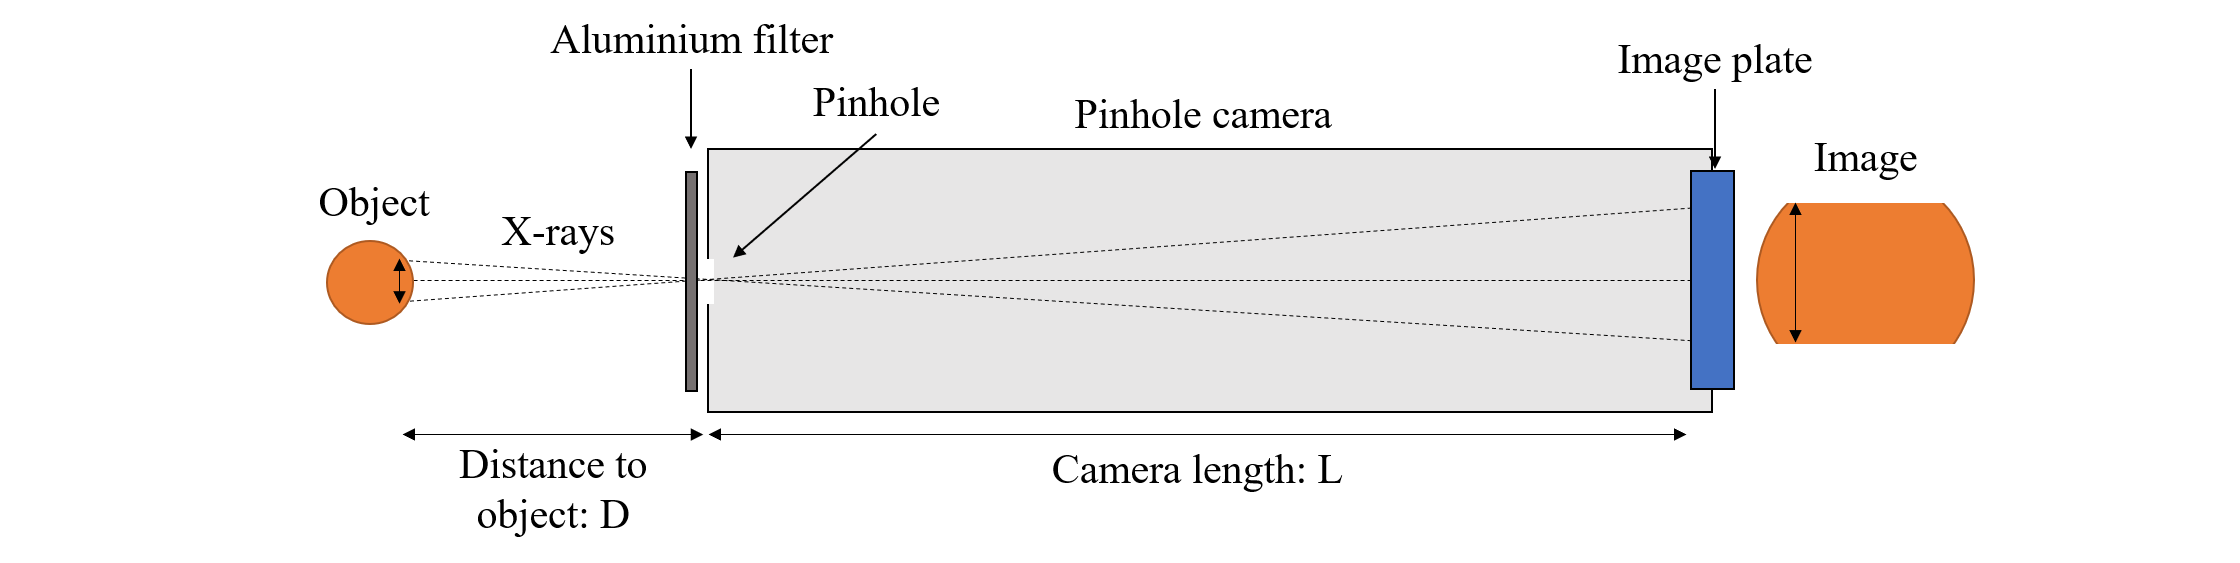
\includegraphics[width=1.0\textwidth]{figures/Experiment/PinholeSchematic2.png}% Here is how to import EPS art
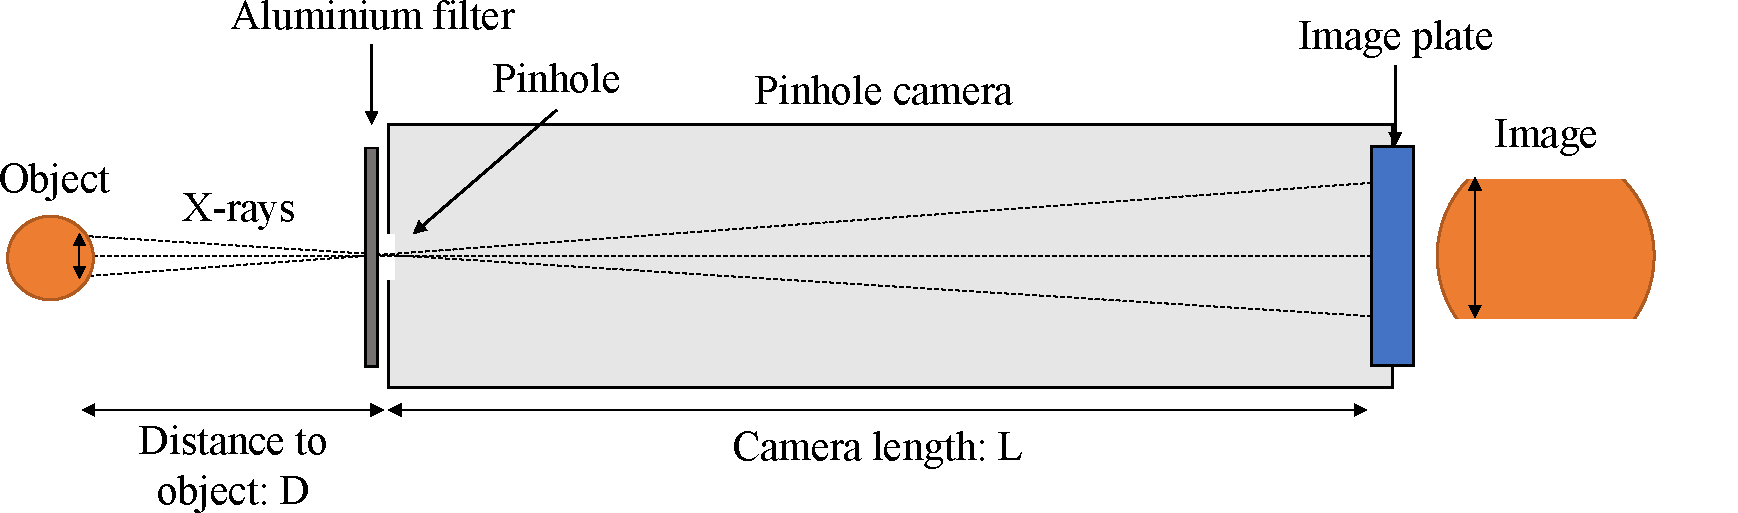
\includegraphics[width=0.8\textwidth]{figures/Experiment/PinholeTest.pdf}% Here is how to import EPS art
\caption{\label{fig:Pinhole schematic} A schematic of a pinhole camera. The distance D between the object and the camera sets the field of view and the magnification.  }
\end{figure}

It is possible to quantify the amount of X-rays received by the image plate, but such an analysis was not necessary/useful for this experiment. Instead, the camera was used to indicate the spatial characteristics of the VULCAN spot. This was useful for confirming where the laser spot hit on the target, that there was a good overlap between the six beams, and to estimate the spot size.

\subsection{Fiducial} \label{Fidu theory}
A fiducial was setup on one of the VISAR streak cameras. A fibre-optic cable was setup behind one of the mirrors in the VULCAN laser chain. These mirrors were slightly lossy, and the fibre `picked-off' some of this parasitic signal. The other end of the fibre was positioned so that it produced a small dot on the side of one of the VISAR streak cameras. The fibre length was such that this parisitic VULCAN signal reached the streak camera in the same streak window that the main signal from the target was detected. This setup can be seen in Figure \ref{fig:Appx-VISARstreaks} in Appendix \ref{app:experimentphotos}.

Two-minute shots (low-power VULCAN shots, so-named as they can be fired every two minutes) were performed without a target present, so that the VULCAN pulse could be measured directly on the streak camera. By doing so, the time delay between the VULCAN shot reaching the target and the fiducial signal showing on the streak could be determined. This meant on subsequent full power shots, where the VULCAN pulse could not be seen directly due to the presence of the target, it was possible to calculate the time at which the pulse was applied based on the fiducial signal.

\subsection{Calorimetry}
Calorimeters, which returned a voltage signal based on the fluence of light received, were in place behind a leaky mirror in each of the six beams. These were calibrated to provide an estimate of the energy in each beam for each pulse (one of these was partly blocked by the fiducial, and so returned a low signal - as the six beams were delivering similar energies, an average of the other beam energies was used for this beam when estimating the total pulse energy).

The VULCAN beam is generated at IR, and had to pass through a frequency-doubling crystal to be converted to 527 \unit{\nano\meter}. The facility staff performed a series of calibration shots. On these shots, larger calorimeters were set up in the main beam path to measure the full energy in each beam, while the orientation of the crystal was optimised. This also allowed for calibration of the smaller, on-shot calorimeters; the voltage the parasitic calorimeters measured as a function of the energy measured by the full calorimeters were recorded, and used to find the relationship between voltage and energy, so that the energy of the beam on shot could be calculated.

\subsection{Pulse length}
Photodiodes were placed behind the final set of mirrors in the Vulcan chain (a different set of mirrors to the calorimeters). This can be seen in Figure \ref{fig:Appx-Photodiode} in Appendix \ref{app:experimentphotos}. These measured the pulse shape of each beam on every shot, and saved it to an oscilloscope - allowing the pulse length and temporal shape of each beam to be observed.

\section{Preparation for the experiment}

\subsection{Development of the optical setup}

An optical setup was required to collect and transmit the self-emitted light to the SOP. Further optics would also be required to transmit the probe laser to the rear of the target, and to collect the reflected beam and deliver it to the VISAR. 

Both VISAR and SOP were operated normal to the rear target surface. While it is possible to operate VISAR off-axis, this has not previously been done in experiments at these intensities (and would also require a correction to the data). Operating both diagnostics in this configuration meant that a shared optical system would be required to transmit the light from the target to the diagnostics, with a dichroic mirror used to separate the 532 nm light from the self-emission. Similar setups are used on Omega \cite{Miller2007, Gregor2016}.

This optical system had to minimise transmission losses to ensure a strong signal at the diagnostics. There was a risk that the self-emission could be relatively weak, and thus it was desirable to avoid placing any beam-splitters in the shared optical relay. This meant that the probe laser injection would need to occur prior to the dichroic mirror, resulting in the basic experiment design displayed in Figure \ref{fig:Simple experiment schematic}.

\begin{figure}
  \centering
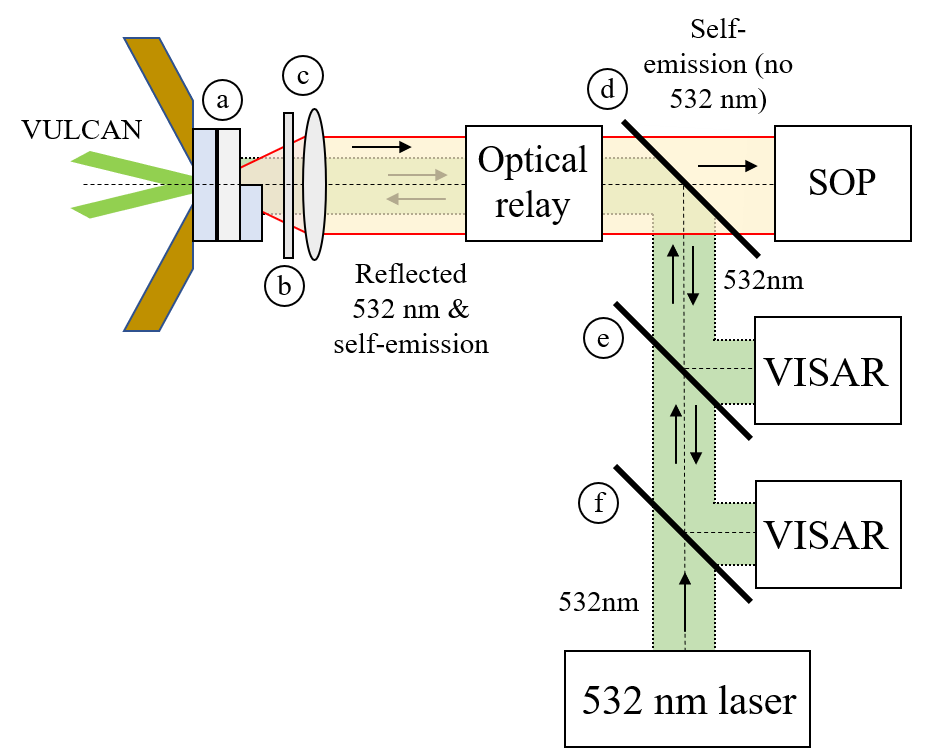
\includegraphics[width=0.6\textwidth]{figures/Experiment/Simple experiment schematic.png}% Here is how to import EPS art
\caption{\label{fig:Simple experiment schematic} A simple schematic of the initially proposed experimental layout. Reflected 532 nm light from a probe laser, and the self-emission, are captured from the target (a) by an objective lens (c) protected by a blast shield (b). This captured light passes through an optical relay, which magnifies it and transports it to the diagnostics. A dichroic mirror (d) reflects the 532 nm light out from the broadband light. This reflected 532 nm light is split and sent to the two VISAR diagnostics via two beamsplitters (e and f). The remaining broadband light passes through the dichroic mirror to the streaked optical pyrometer. The 532 nm laser is injected through the back of the second VISAR beamsplitter, and travels through the full optical relay to illuminate the target. This setup avoids the need for the self-emission to pass through a beamsplitter on it's route from the target to the SOP.  }
\end{figure}

A number of factors needed to be considered in the design of this system:

\begin{itemize}
    \item \textbf{Optical relay spacing}: The spatial configuration of the target chamber and area set limits on the optical relay design. Injecting the probe laser through the VISAR beamsplitter required the laser to be located relatively close to the diagnostics (to avoid a long beam path around the target area). This set constraints on the positions of the optical benches in the target area, and meant that it would be necessary for the optical relay to transmit the light through the south chamber window (which was furthest from the target position). This window was 1.5m away from the target position, with a further 1.3m of window/free space propagation before the optical table would be reached.
    
  \begin{figure}
  \centering
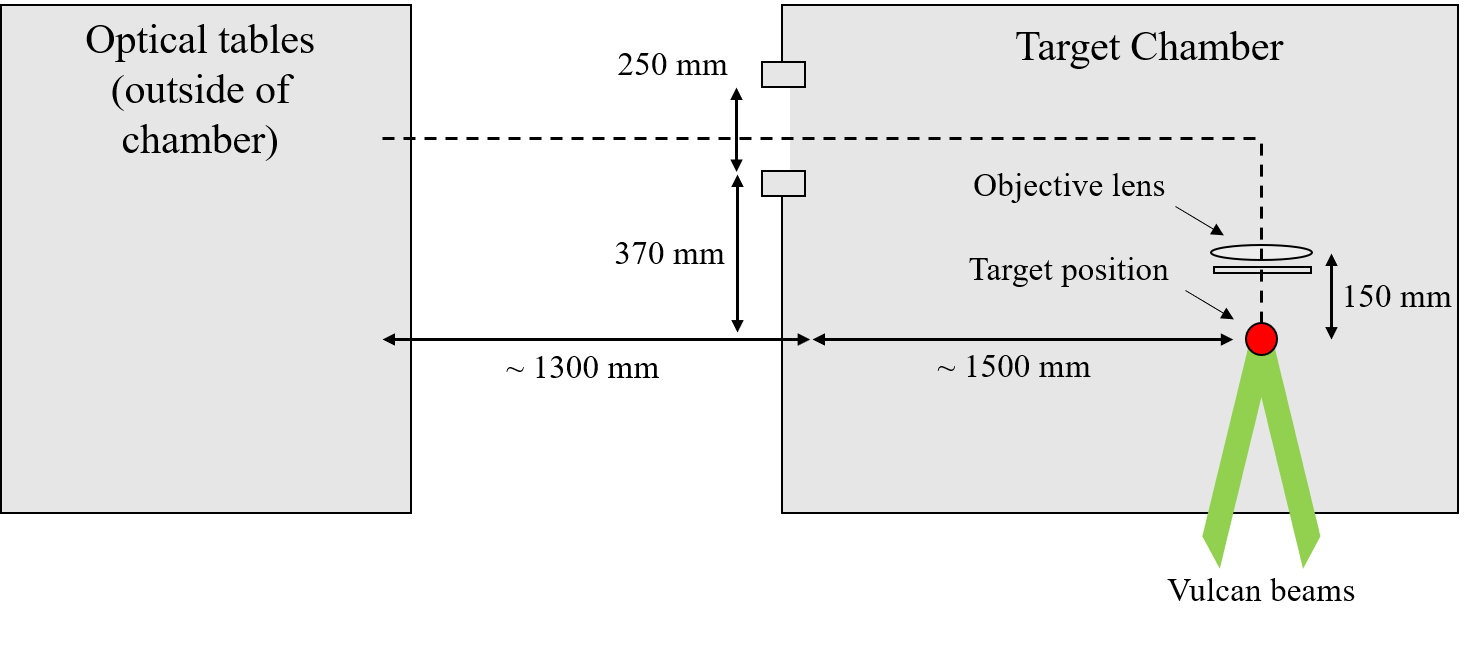
\includegraphics[width=0.8\textwidth]{figures/Experiment/Experiment Spacing.png}% Here is how to import EPS art
\caption{\label{fig:Experiment} A simple schematic (not to scale) showing the spacial considerations for the optical relay. There was a useable distance of $\sim$ 1500 mm of optical table within the chamber before the window. There was then a further $\sim$ 1300 mm gap (in which no lenses could be placed) before the optical tables outside of the chamber, which housed the diagnostics. }
\end{figure}  
    
    \item \textbf{Magnification}: The SOP streak camera had a slit width of 4.46 \unit{\milli\meter}, while the VISAR streaks both had a width of 17.4 \unit{\milli\meter}. The imaged area was 400\unit{\micro\meter} in diameter, and should be magnified to fill as much of the camera slit as possible. The VISAR already had a number of built in lenses (of which only the first could be changed), and so it was necessary to design a system which would provide appropriate magnification for both diagnostics as well as transmitting the beams with minimum losses over the relevant distances.
    
    \item\textbf{Components}: The optical components required for the relay and for the diagnostic systems also needed to be identified and purchased. This included: a dichroic mirror, low-pass and high-pass filters for the SOP, and notch filters (to prevent any 527nm Vulcan noise affecting the VISAR signal). Many of these components, as well as the optical components within the VISAR, were only available in 1-inch versions - which set limits on the beamsize.
    
    \item \textbf{Diagnostic positioning}: Finally, it was necessary to consider how the diagnostics and beam paths would actually fit on the optical table. The VISARs in particular were large pre-assembled systems with fixed entry points for the beam path. The 1-inch optical components meant it was necessary to minimise the distances between the VISARs and the final lens in the optical relay to avoid transmission losses, but this was challenging to achieve practically.
    
\end{itemize}

To assist with this design work, a Matlab script was produced to perform ray-tracing (using simple geometrical optics) of light through a lens system. A number of setups were explored using this code to find a system which minimised losses while being compatible with the above considerations. The final design achieved this, with transmission (according to the simple approximations used within the code) above 99\% from the first lens to the target. Details of the operation of this code are provided in Appendix \ref{appdx: Ray Tracing}.

Figure \ref{fig:Full experiment schematic} shows a full schematic of the experiment. The optical relay consists of 5 lenses (L1 to L5). The dichroic mirror then takes the collimated beam, and sends the signal to the SOP/VISARs. The SOP consists of a 400 nm long pass filter and 500 nm short pass filter, leaving only 400 - 500 nm wavelengths, before a final lens S1 focusses the beam on to the streak camera. Beamsplitters send the VISAR beam into the VISAR system (the `VISAR' here is used to refer to the full system shown in Figure \ref{fig:Dan_VISAR}, rather than just the interferometer). The beam passes through a notch filter, followed by the 4 lenses within the VISARs (and the interferometer, which is not shown), before being focussed onto the beam splitter by lens V5 (and further focussed in the vertical direction by the cylindrical lens V6). The lens spacing can be seen on the CAD models in the appendix. The spacing between focussing pairs is fixed by the focal distances of the lenses. There was some flexibility in the spacing between L1 \& L2 and L3 \& L4; however, the distance between L5 \& V1 for each VISAR had to be kept below 1m to avoid losses (otherwise the beam would be too large for the 1 inch components inside the VISAR), and the distance from V4 to the VISAR streak camera also needed to be under 1m. The short pass filter (c) was also a 1 inch component, and so it was important to place this close to the dichroic mirror.

\begin{figure}
%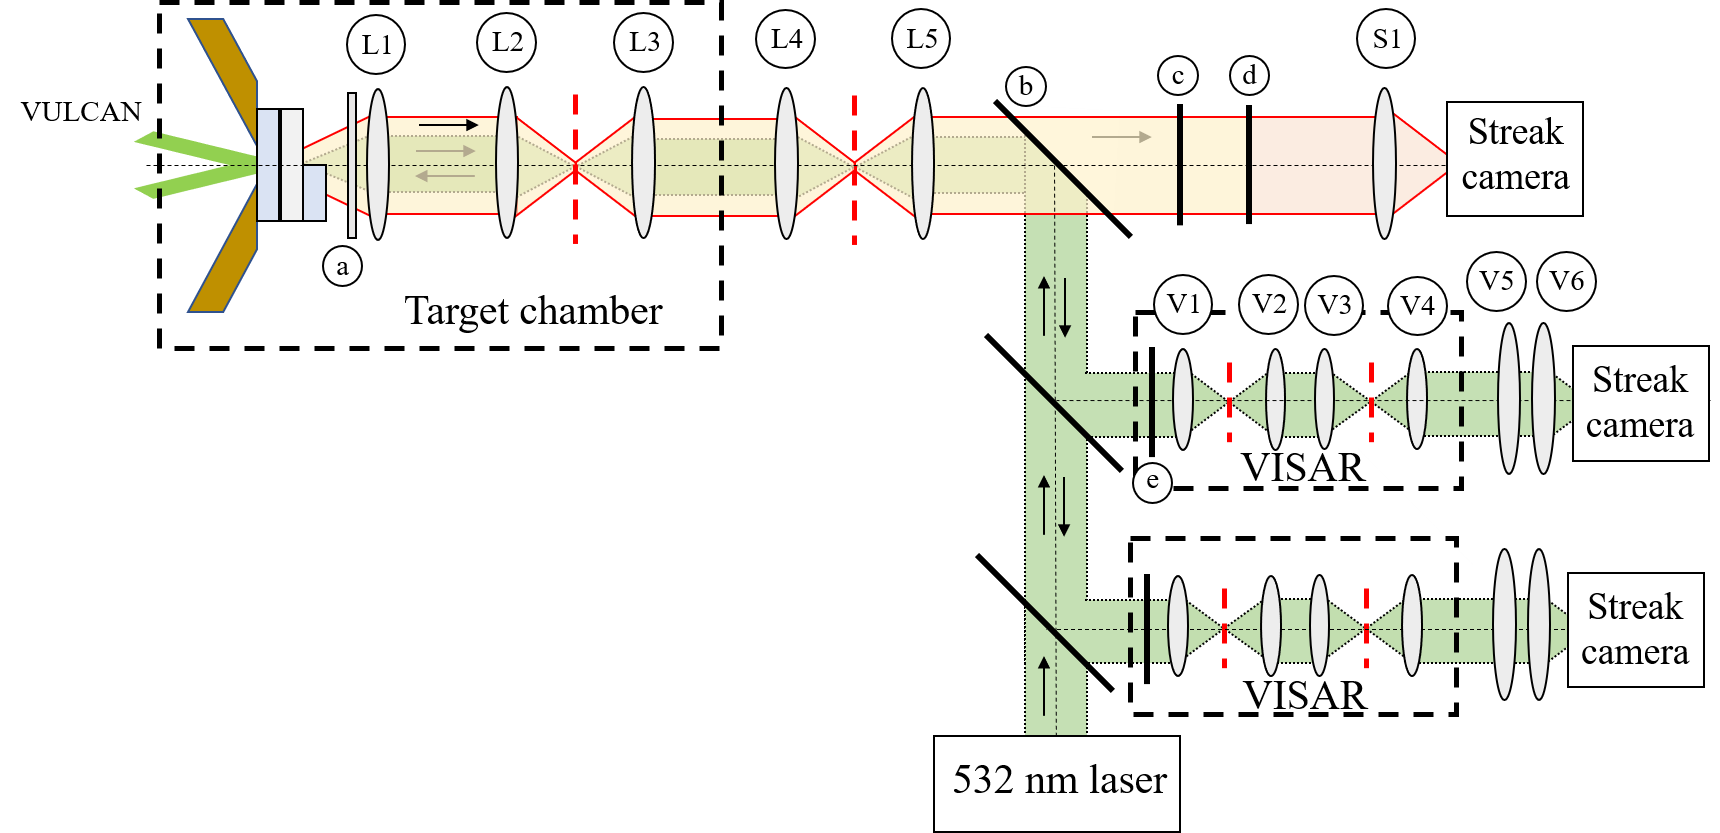
\includegraphics[width=1.0\textwidth]{figures/Experiment/Full experiment schematic.png}% Here is how to import EPS art
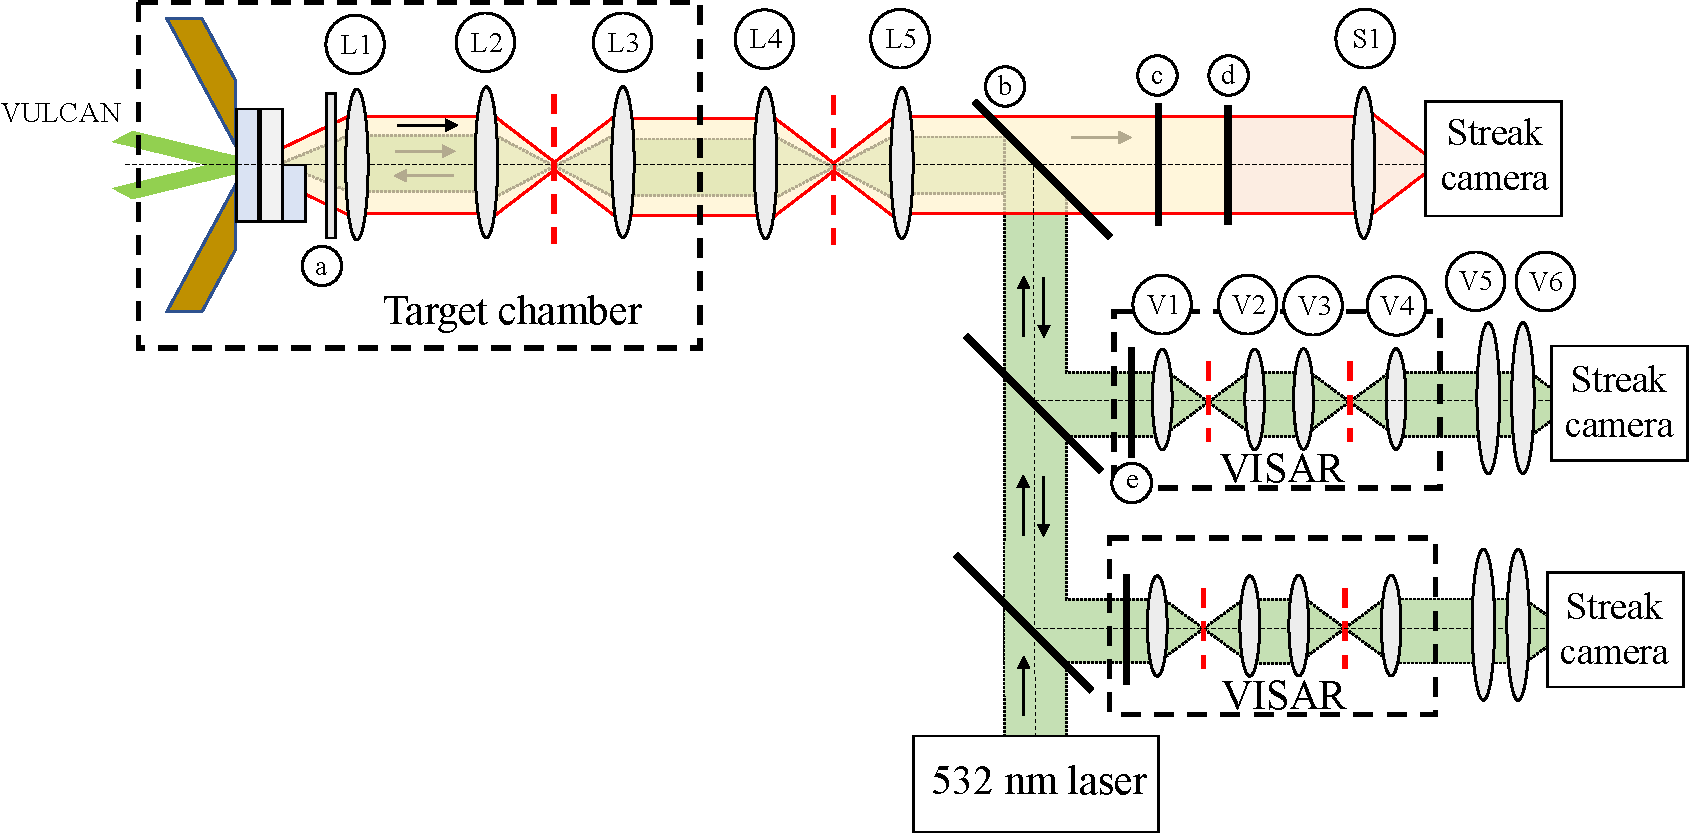
\includegraphics[width=1.0\textwidth]{figures/Experiment/Full Experiment Schematic.pdf}% Here is how to import EPS art
\caption{\label{fig:Full experiment schematic} The full proposed schematic. Lenses labelled 'L' form the optical relay, while those labelled 'S' are part of the SOP and 'V' are part of the VISAR. The two VISARs are identical in terms of components. The dashed red lines represent the positions of image planes. The interferometer in the VISAR is not pictured (it can be viewed in Figure \ref{fig:Dan_VISAR}), but is positioned so that the second beamsplitter is positioned at the second image plane. The focal lengths are as follows: L1 = 150mm, L2 = 700mm, L3 = 500mm, L4 = 700mm, L5 = 250mm, S1 = 300mm, V1 = 400mm, V2 = 250mm, V3 = 1000mm, V4 = 300mm, V5 = 300mm, V6 = 200mm (cylindrical). Also indicated are the other components in the beamline: a blast shield to protect the objective lens (a), the dichroic mirror (b), the short-pass (c) and long-pass filters (d) for the SOP, and notch filters (e) for the VISARs.}
\end{figure}

Figure \ref{fig:Original CAD} shows the designed arrangement of this setup, which allows all the spatial requirements to be satisfied. Figure \ref{fig:Ray trace} then shows the output of the ray tracing script for the target to SOP and target to the second (furthest) VISAR. 

\begin{figure}
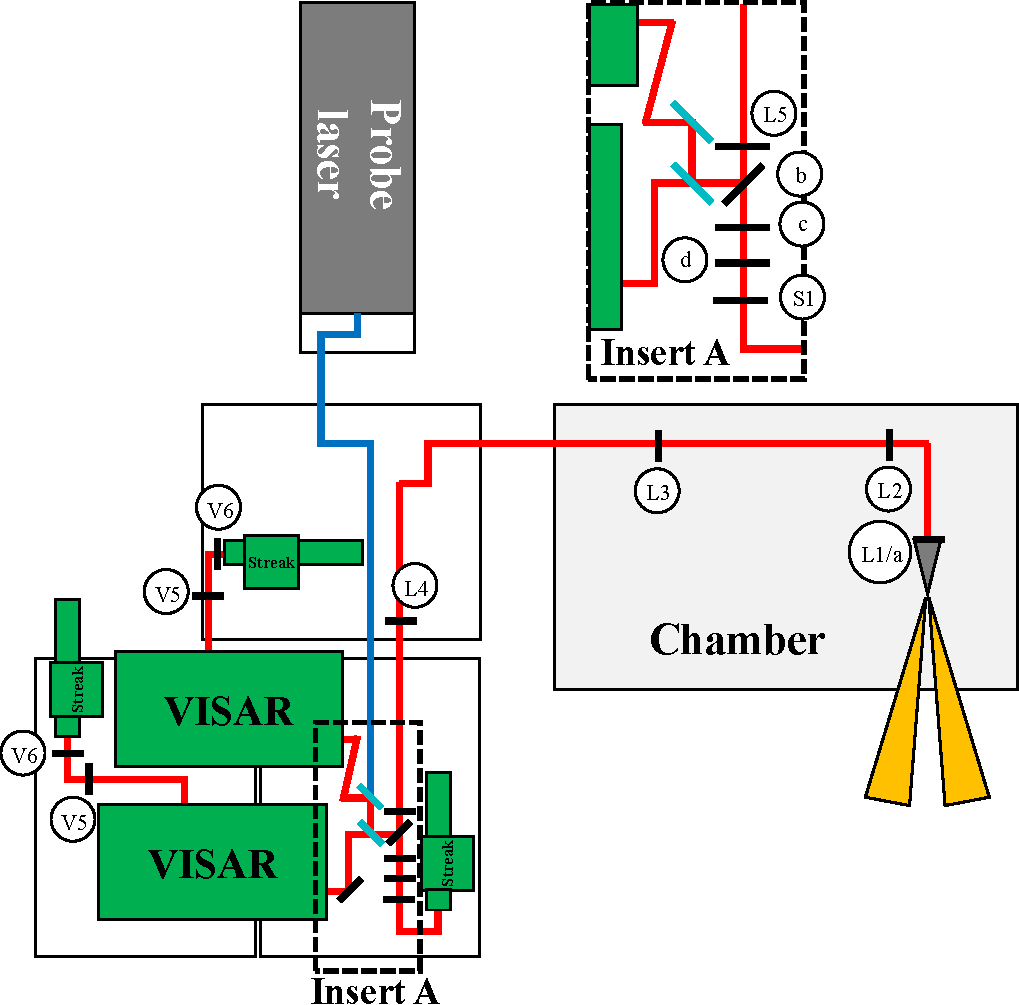
\includegraphics[width=0.8\textwidth]{figures/Experiment/OriginalSetup.pdf}% Here is how to import EPS art
\caption{\label{fig:Original CAD} A schematic showing the spatial arrangement of the experimental equipment (not quite to scale, but close enough to be representative). The white boxes indicate the optical tables on which components could be placed. Mirrors are not shown, but are present when the beam turns. Beamsplitters are displayed in teal; all other components are labelled as described in Figure \ref{fig:Full experiment schematic}. The insert shows a close up view of the section in the dashed black box. The beamline colors are used to correspond to the CAD models in the appendix, rather than representing anything physical.}
\end{figure}


\begin{figure}
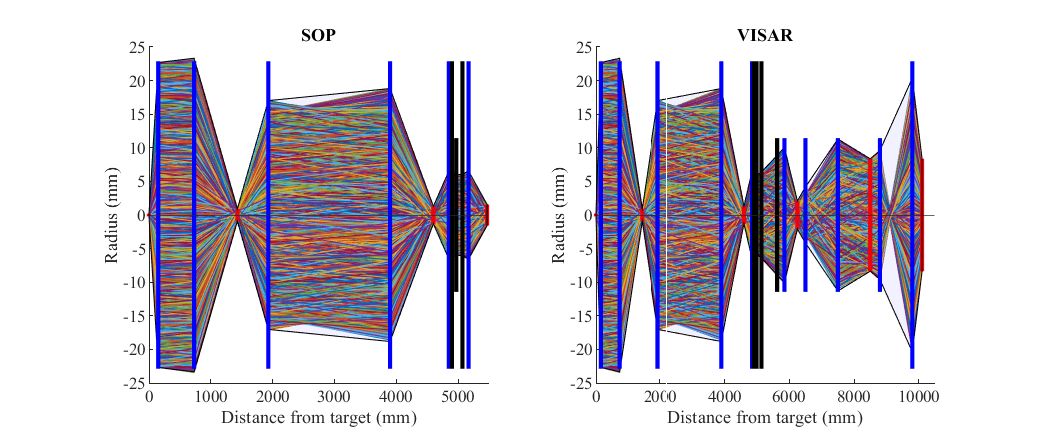
\includegraphics[width=1.0\textwidth]{figures/Experiment/RayTracing.eps}% Here is how to import EPS art
\caption{\label{fig:Ray trace} Ray tracing simulations from the target through to the SOP and VISAR. The components are placed with the real experimental spacing. Lenses are represented by blue lines, while other components (dichroic mirror, beamsplitters, filters) are represented by black lines. 10,000 rays are generated, each at a random position on the target and with a random angle. These rays are propagated through the system according to simple geometric optics through thin lenses. At each component position, the radial position of each beam is compared to the component size; if it is bigger, the ray is considered `lost'. This approach suggests transmission through the system greater than 99\% for both the VISARs and SOP (with the small losses occuring between L1 and L2).}
\end{figure}

\subsection{Target design and hydrodynamic simulations} \label{Target Design}

\subsubsection{Layer choice and thickness}

The target was based on multi-layer step target desgins successfully used in previous experiments \cite{Falk2014a, Falk2020}. The initial proposal used an aluminium layer as the reference, but this was replaced with quartz so that the velocity of the shock could be measured directly using the VISAR \footnote{The original proposal had suggested that the VISAR could be used to measure the free surface velocity of the aluminium and foam. Under this approach, the VISAR reflects from the rear of an opaque target. The target is shocked, and the shockwave reaches the rear surface, which undergoes free surface expansion. The free surface velocity is measured by the VISAR; this is generally approximated as being twice the particle velocity within the shocked medium. This is a common approach at lower pressures, but it is not possible in this regime - as the shocked material becomes a plasma, the rear surface is destroyed and thus the free surface velocity cannot be measured. As such, the target design was changed to replace the aluminium with quartz, and the foam shock velocity was instead determined from the transit time}. The four layers and step structure led to a relatively complicated target.

The thicknesses of the different layers were influenced by a number of factors. These are listed below:

\begin{itemize}
    \item \textbf{VULCAN pulse length/energy capabilities}: In order to ensure a sustained shock, it was intended that the laser pulse should last until the shock broke out from the rear of the target. There was an upper limit on how long VULCAN could sustain a pulse for (particularly at high intensity, where high energy is required), and this therefore prevented very thick targets with long shock propagation times.
    \item \textbf{Secondary shocks}: Hydrodynamic simulations showed that when the shock crossed from the gold layer into the quartz, a release wave would propagate back through the target. Upon reaching the ablation front, this would generate a second shock which would travel through the target. Depending on intensity/target thickness, this secondary shock could catch up and merge with the primary shock. This would mean the shock strength would change, which would prohibit the use of the impedance matching calculation. This effect was heavily influenced by the thickness of the different layers, and needed to be avoided. An example of this behaviour can be seen in Figure \ref{fig:ShockPlot}, in Chapter \ref{ch-experimentAnalysis}.
    \item \textbf{Fabrication constraints}: Target fabrication indicated that the 40~\unit{\micro\meter} was the minimum thickness of quartz/foam that they would be able to produce.
    \item \textbf{Preheating}: The gold layer would need to be sufficiently thick to prevent preheating of the quartz/foam. 
    \item \textbf{Avoiding direct laser heating of gold}: The ablator needed to be sufficiently thick so that the ablation front remained in this layer throughout the laser pulse, and thus the gold did not undergo direct laser heating.
\end{itemize}

HYADES simulations were performed to find the optimal target design. The minimum 40~\unit{\micro\meter} thickness for the quartz and foam was chosen to mitigate the pulse length concerns. This also was required for the second shock; the thicker the quartz/foam layers were, the more distance there was for the second shock to catch the primary shock in. Even for 40~\unit{\micro\meter} quartz/foam thickness the second shock was already a significant problem. 

Increasing the gold and ablator thicknesses were both found to delay the second shock, improving this issue (the gold/quartz interface was moved further from the ablation front, which meant the second shock (which has to travel this distance twice once it is generated at this interface) had a longer distance to travel relative to the first). Simulations were performed investigating the potential gold/ablator thicknesses that could be used, and the impact this would have on the required laser pulse time/energy at different intensities.

The selected design used a 40~\unit{\micro\meter} ablator, and a 3~\unit{\micro\meter} gold layer. In Hyades, this led to the required pulse times/pulse energies as a function of intensity seen in Figure \ref{fig:VULCAN energy} - remaining under the 600 J maximum energy of VULCAN for the full planned intensity range \footnote{In the spherical hydrodynamic simulations in Chapter \ref{ch-lowCR} a multiplier is applied to the incoming laser energy to account for losses. These are likely reduced for this setup, but some losses would still be expected. The simulations presented in this section do not include such a multiplier, and so it's likely that the shots would require a larger energy/pulse time for a given intensity. However, as the highest intensity in Figure \ref{fig:VULCAN energy} requires only 500 J as opposed to the 600 J VULCAN can deliver, there is some additional energy available to account for this. }. The target did not experience second shock merger over this intensity range. The simulations also suggested that the ablation front remained in the ablator for all of these intensities, and that the 3\unit{\micro\meter} gold layer would prevent preheating of the foam to less than 10K. Hydrodynamic simulations cannot be expected to describe preheating with high accuracy, as they do not include many of the laser plasma effects; however, previous experiments have used similar gold thicknesses and did not report substantial amounts of preheat, suggesting that this thickness is likely sufficient.


\begin{figure}[hbt!]
\centering
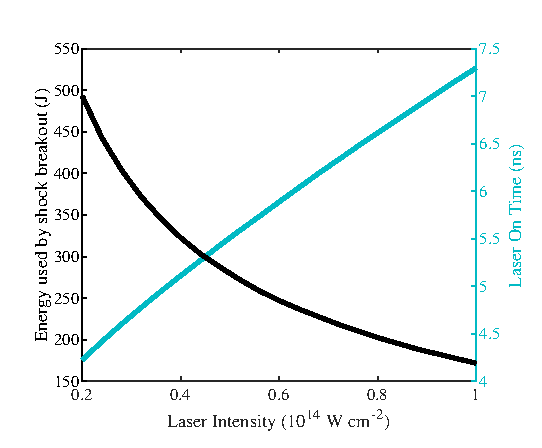
\includegraphics[width=0.6\textwidth]{figures/Experiment/EnergyandPulsetimes_edit.eps}% Here is how to import EPS art
\caption{\label{fig:VULCAN energy} The required VULCAN pulse times as a function of intensity, if the pulse is to be applied until shock breakout from the rear of the target, as simulated in HYADES. The shock breakout time is identified from simulation at each intensity, which defines the required pulse time. The energy of this pulse (given the known intensity and required pulse time) can also then be calculated. There is an inverse relationship between these two parameters; higher intensities result in faster shocks (and thus shorter required pulse lengths), but the increased intensity also means that the required energy of the pulse is higher (i.e. the pulse length does not reduce by enough to balance the increased power).}
\end{figure}

\subsubsection{Additional considerations}

There were also a number of practical concerns with the target assembly. Firstly, it was key to the experiment that no glue layers were used in the target, for a number of reasons. Firstly, there was concern that glue might wick into the foam, which would change it's behaviour. Secondly, a glue layer between the quartz and the foam would prevent impedance matching being performed, as the shock would need to pass through the glue layer. Finally, a glue layer between the gold and the quartz would make it difficult to determine when the shock entered the quartz from the glue layer. This meant that the target had to be constructed without glue. The manufacture of the targets was handled by CLF target fabrication (particularly Chris Spindloe, Sam Irving, David Haddock, and Donna Wyatt). The ablator and gold coatings were grown directly on to the quartz, so that no glue was required here. The foam was placed in position on the quartz, so that one foam edge was centered on the quartz piece (giving the step structure). The foam was then `tacked' to the quartz with glue at the corners - this was sufficiently far from the center of the target that there would be no glue between the layers in the shocked/imaged region.

Secondly, coatings were required for the quartz. An anti-reflection coating was requested on the quartz surfaces, to prevent spurious reflections and `ghost fringes' (where reflections from other surfaces lead to interference and persistent fringes in the data).

\subsection{Hydrodynamic simulations}

The hydrodynamic simulations mentioned in the previous section also enabled the expected conditions in the quartz/foam to be investigated. A selection of the key shock variables can be seen in Figure \ref{fig:PreExpHydro}. These simulations were performed in Hyades and were used to inform etalon selection, as well as confirming that the quartz pressure was sufficient for a reflective shock front. Experimental collaborators also ran simulations of this in Multi, Helios, and FLASH, and good agreement was observed (a comparison between these codes can be seen for post-experiment simulations in Figure \ref{fig:SimulationPlot} in Chapter \ref{ch-experimentAnalysis}).

\begin{figure}[hbt!]
\centering
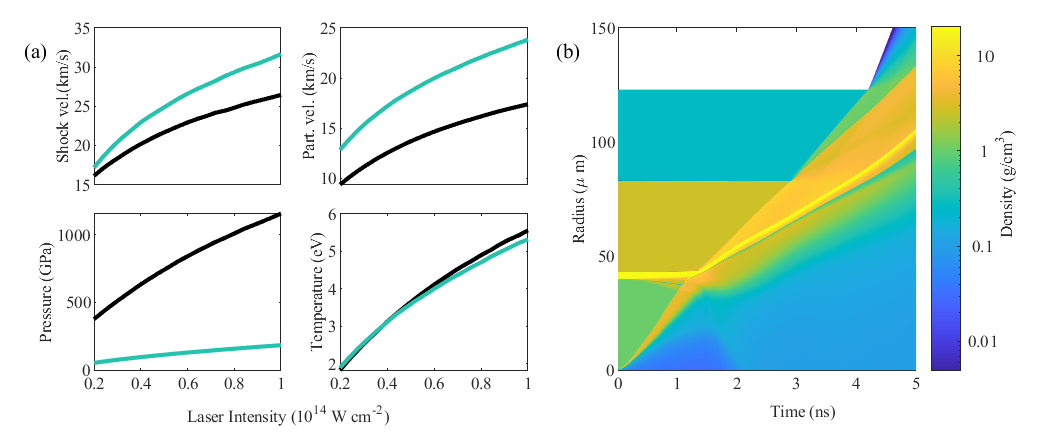
\includegraphics[width=1\textwidth]{figures/Experiment/PreExperimentHydro.eps}% Here is how to import EPS art
\caption{\label{fig:PreExpHydro} Shock conditions in the quartz (black) and foam (teal) as a function of intensity (a), and a density plot showing shock propagation through the target for an intensity of \num{1e14} \unit{\W\per\centi\meter\squared}. The quartz shock velocity informed decisions on the required etalons. The shock pressure in the quartz is also confirmed to be above the threshold for a reflective shock for the full range of simulated intensities.}
\end{figure}

Two-dimensional simulations of this setup were also performed to ensure that the shock was planar and that similar shock behaviour was observed in higher dimensions. The simulations presented in this section were performed in h2D (the two-dimensional version of Hyades). This is a Lagrangian code and as such suffers from mesh tangling, where the movement of the different zones can cause the mesh to become distorted and prevent the simulation from continuing. This requires the user to manually rezone the problem, and frequently also resulted in the simulation code crashing. After a number of iterations a sufficiently detailed simulation was ran to completion. Other 2D simulations were performed in Multi-2D and FLASH 2D by the other collaborators and were used to confirm these results; as these codes were ran with more success they were used instead of h2D for the post-shot simulations, and will be discussed in more detail in that section.

In h2D, a simple four layer target was simulated without a step in the foam. This was sufficient to measure shock propagation and to estimate the shock variables, as well as to indicate the shock planarity. 2D FLASH simulations were used to confirm that the step did not have a significant impact on the shock behaviour (a post-shot 2D Flash simulation with this structure is shown in Figure \ref{fig:SimSubPlot} in Chapter \ref{ch-experimentAnalysis}). h2D is an axisymmetric code, and so the target is simulated as a cylinder where the shock propagates along the long axis. R=0 is the axis of symmetry, and the 2D plane can be rotated around this axis to produce the full target (this also means that any off-axis represent rings of laser light when extruded to 3D). The lasers were simulated as 3 beams at -25$^{\circ}$, 0$^{\circ}$, and 25$^{\circ}$ to the target normal. Given the real experimental configuration (three pairs of two beams) a simulated setup consisting of two beams at 6$^{\circ}$ and -6$^{\circ}$ would also have been valid, but the three beam setup was chosen as it included larger deviations from target normal, and would thus be more likely to exhibit changes from 1D behaviour. 

Figure \ref{fig:H2DSchematic} shows a number of schematics representing the simulated setup, and how it compares to the real experimental configuration. Figure \ref{fig:H2DSchematic} (a) shows the real laser setup (not to scale), with the true 3D configuration of the six beams. This cannot be fully described in 2D. Figure \ref{fig:H2DSchematic} (b) shows the 2D simulation. Three laser beams are simulated by specifying a number of `rays' with an initial angle and position. The rays were created using a `random-to-uniform' lens-to-target mapping in Matlab. 10,000 uniformly spaced points were generated over the laser spot at the target, and for each point an incident ray was generated. Each ray was given an origin position at random, corresponding to a position on the lens for one of the three laser beams (considering the real lens size and lens-to-target distances). This method ensures that uniform illumination of the laser spot is achieved with the finite number of beams, while also using a random mapping to ensure behaviours such as defocussing past the laser focus. The energy of the ray was scaled according to the square of it's radial position at the target; this accounted for the axisymmetric symmetry, and the fact that a ray incident on a higher radial position is spread over a much larger area if the 2D slice is converted to a 3D cylinder. While only positive radii are simulated, as the rays are described at a single point (on the target face), it is possible to include rays which would have originated on the other side of the Z-axis. This is shown in Figure \ref{fig:H2DSchematic} (c) where the simulation is reflected around the z axis, and it is shown that the rays shown in (b) do in fact originate from all 3 beams. Finally, Figure \ref{fig:H2DSchematic} (d) shows the rotation of the simulated setup in (b) around the axis. Here, it can be seen that this rotation means that the off-axis beams in fact represent a hollow cone of incoming laser light.

%\begin{figure}[hbt!]
%\centering
%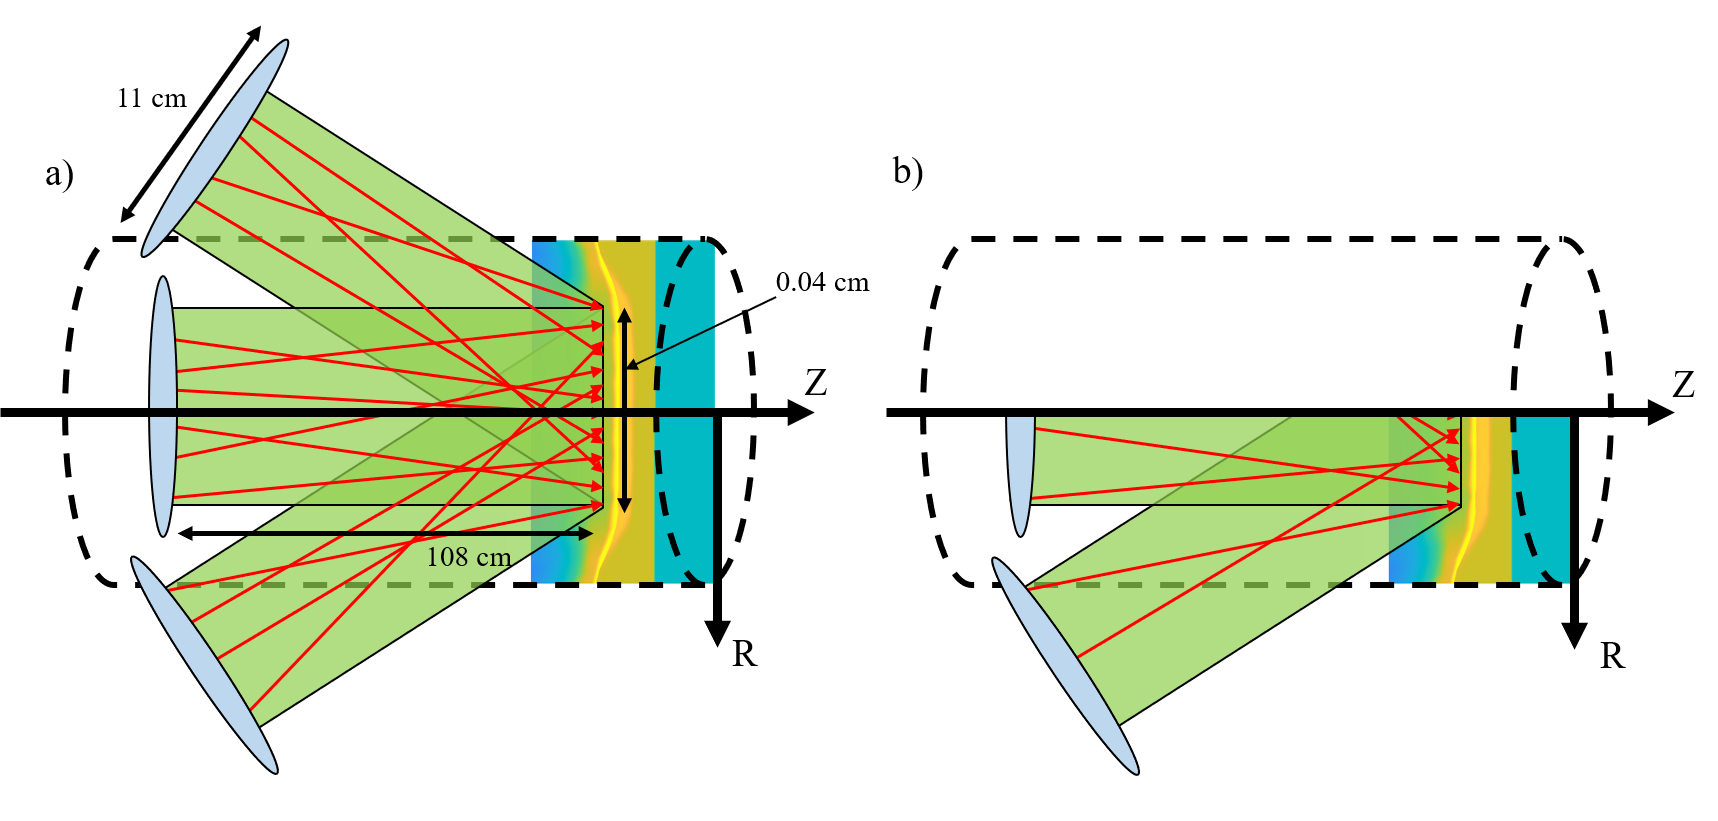
\includegraphics[width=1\textwidth]{figures/Experiment/H2DSchematic2.png}% Here is how to import EPS art
%\caption{\label{fig:H2DSchematic} A schematic (not to scale) showing the simulated setup. In a), the full concept is shown. Three three beams produce a 400 \unit{\micro\meter} laser spot on the target. These beams are described by a series of rays originating from three 11 cm diameter lenses 108 cm from the target (these dimensions are accurate to the experiment). A small number of example rays are demonstrated by the red arrows. The rays are evenly spaced at the laser spot, but each is mapped to a random origin point on one of three lenses, which ensures the beam would defocus appropriately beyond the focal plane (the lenses are much larger than the focal spot, and so in practice these beams are heavily focussed - unlike in the schematic). For the purposes of the simulation, the target is considered to be a cylinder. R and Z are simulated, but the azimuthal behaviour is neglected (due to the 2D nature of the simulation). In b), the section included in the simulation is shown. Half the target diameter is simulated, and this can be extruded round the azimuth to produce the full target. Only the rays incident on this half of the target are included - but as the rays are specified at the target surface, it is possible to include rays that would have originated on the other side of the Z-axis. As the rays would also be uniform around the azimuth, the two off-axis beams would actually be simulated as a cone of incoming laser light.}
%\end{figure}

\begin{figure}[hbt!]
\centering
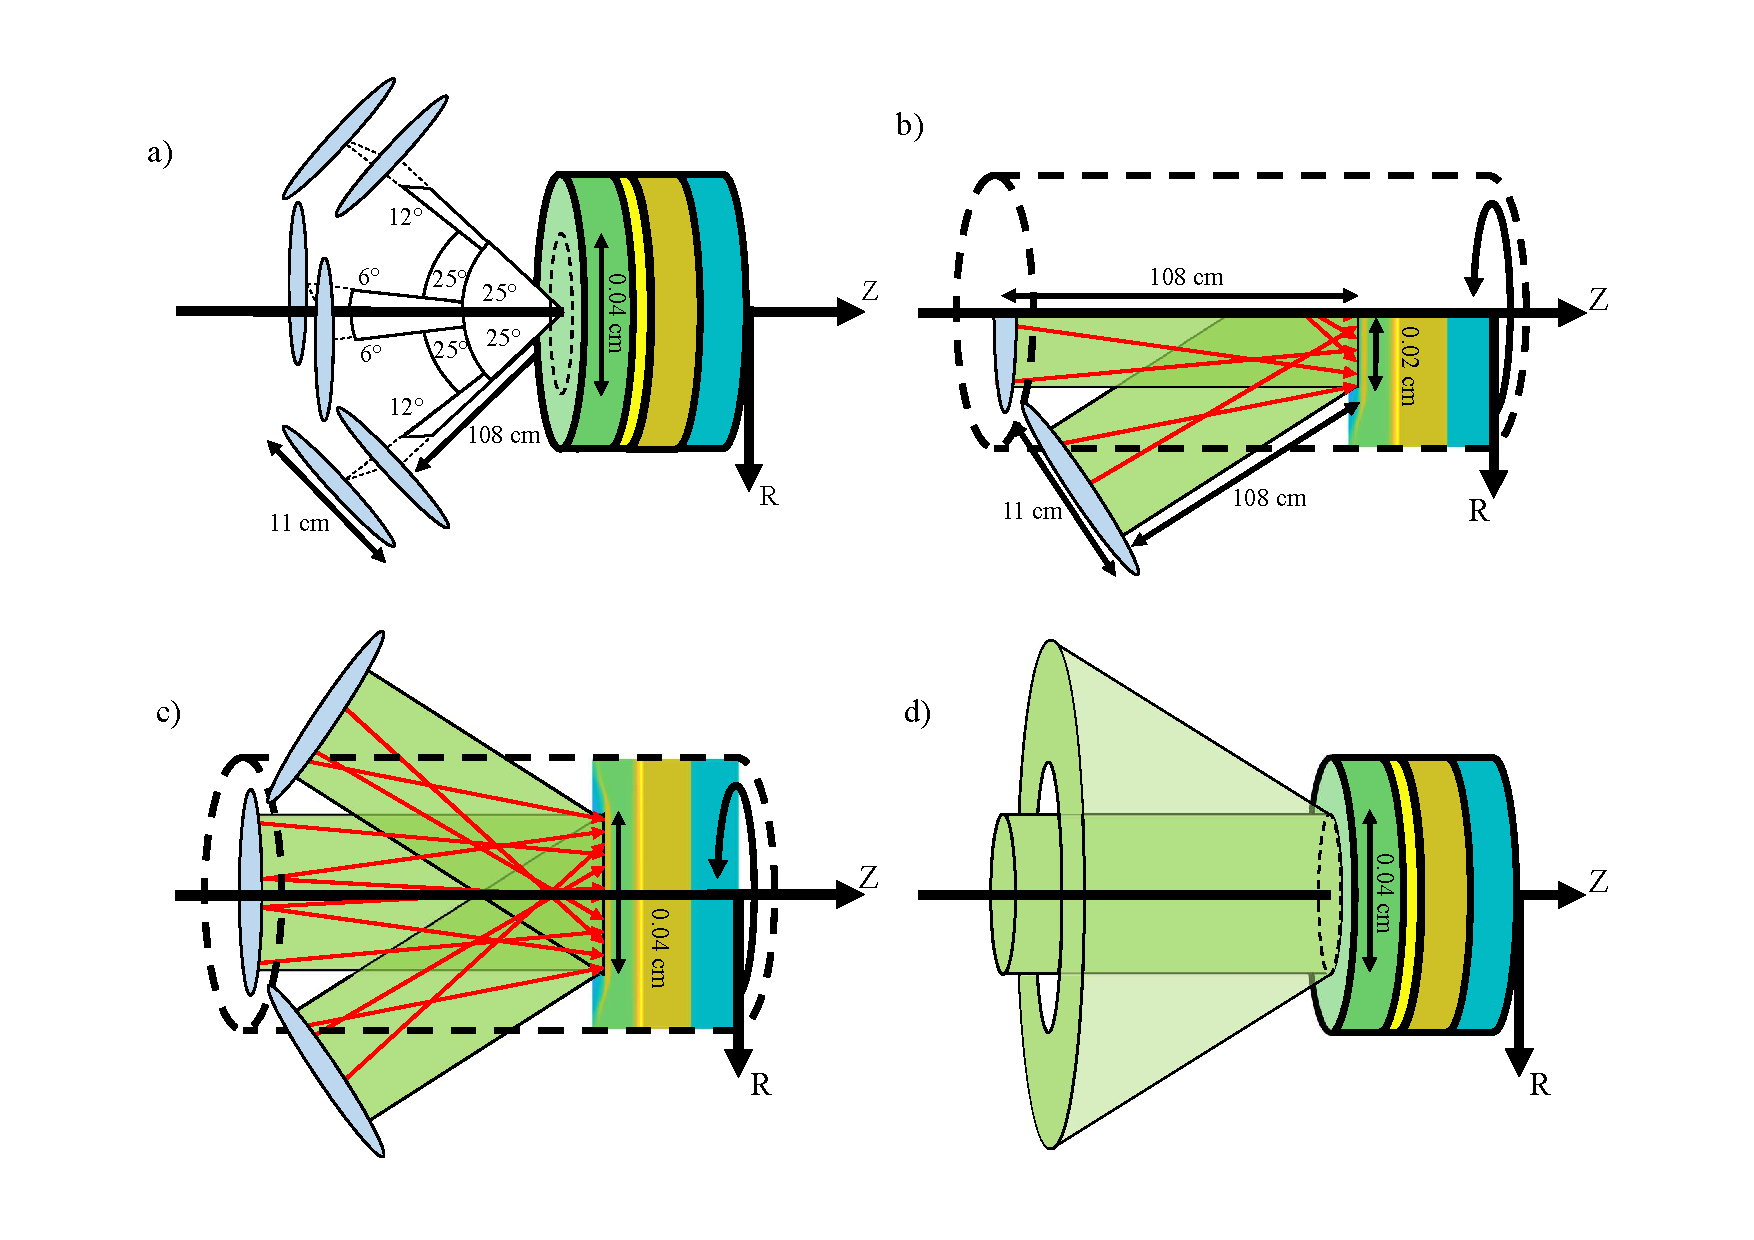
\includegraphics[width=1\textwidth]{figures/Experiment/H2DSchematic.pdf}% Here is how to import EPS art
\caption{\label{fig:H2DSchematic} A schematic (not to scale) showing how the setup is simulated in h2D. a) The real experimental layout of the 6 beams. The beams are arranged in three planes at -25$^{\circ}$, 0$^{\circ}$, and 25$^{\circ}$ to the horizontal, with each plane containing two beams at 6$^{\circ}$ and -6$^{\circ}$ to the vertical. Each beam is 11 \unit{\centi\meter} in diameter at the lens, which is 108 \unit{\centi\meter} from the target, and is focused to a 400 \unit{\micro\meter} meter spot. b) The h2D simulation. This is done in 2D with cylindrical symmetry. The laser is described using rays, which are mapped from a random position on one of three lenses (at -25$^{\circ}$, 0$^{\circ}$, and 25$^{\circ}$ to the horizontal, at the correct distance) to a uniform grid of points in the laser spot. c) The h2D simulation has been reflected around the x-axis, and the rays traced back to show their sources. As the rays are generated in the laser spot, the configuration in (b) allows for rays to cross the z-axis, even though this lens would not be in the area included in the simulation. d) The 3D extrapolation of the 2D simulation. As the simulation has cylindrical symmetry, the two beams at -25$^{\circ}$ and 25$^{\circ}$ actually form a laser `ring', with a hollow cone of incoming laser light.}
\end{figure}

Figure \ref{fig:H2DPlot} (a) shows four snapshots of the 2D shock structure. It can be seen that the shock front is relatively planar over a nearly 200 \unit{\micro\meter} radius (and thus the 400 \unit{\micro\meter} diameter of the imaged region). Figure \ref{fig:H2DPlot} (b) shows the shock propagation through the target (at the position of the dashed black lines in (a)) as a function of time, which shows good qualitative agreement with the 1D simulation seen in Figure \ref{fig:PreExpHydro}.

\begin{figure}[hbt!]
\centering
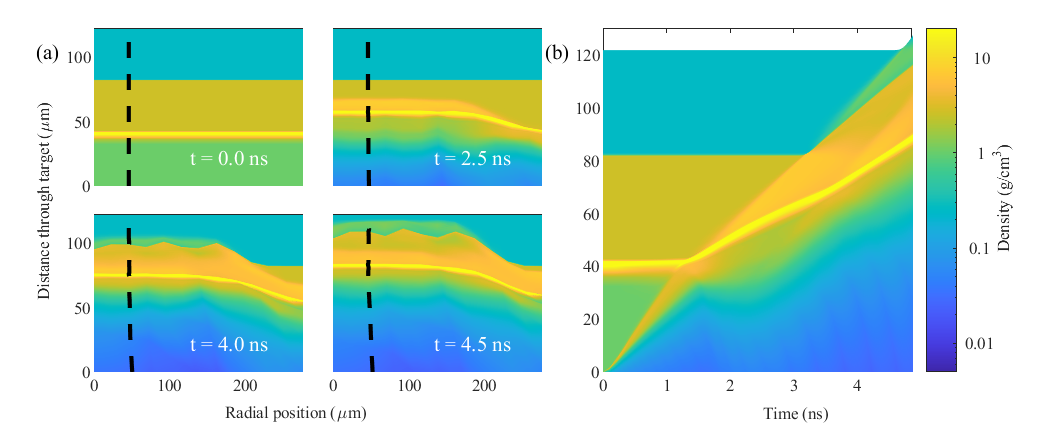
\includegraphics[width=1\textwidth]{figures/Experiment/H2DPlot.eps}% Here is how to import EPS art
\caption{\label{fig:H2DPlot} A two-dimensional h2D simulation of the setup using a simple four-layer target (ablator, gold, quartz and foam without the step structure), for a laser intensity of \num{1e14} \unit{\W\per\centi\meter\squared}. (a) shows four snapshots of the 2D simulation at the indicated times, while (b) shows the shock propagation of through the target as a function of time for a given radial position, represented by the black dashed lines in (a). It can be seen that for the later two times, the black dashed line is noticeably curved. This is because the lagrangian mesh moves as the simulation occurs, and thus the mesh points (where the simulation parameters are returned) do not have fixed radii. This small amount of curvature does not significantly affect the results - particularly as it is only seen in the ablated material significant behind the shock.}
\end{figure}

Figure \ref{fig:H2DPressure} shows how the pressure just behind the shock front in this simulation varies across the radius of the target. It is clear from the figure that, while the pressure reduces towards the edge of the target, over the central region the shock pressure is relatively planar in both the quartz and the foam. Meanwhile, Figure \ref{fig:H2DTiming} displays the shock breakout times from the gold, quartz and foam layers. This again indicates that the shock is planar over the central region of the laser spot.

\begin{figure}[hbt!]
\centering
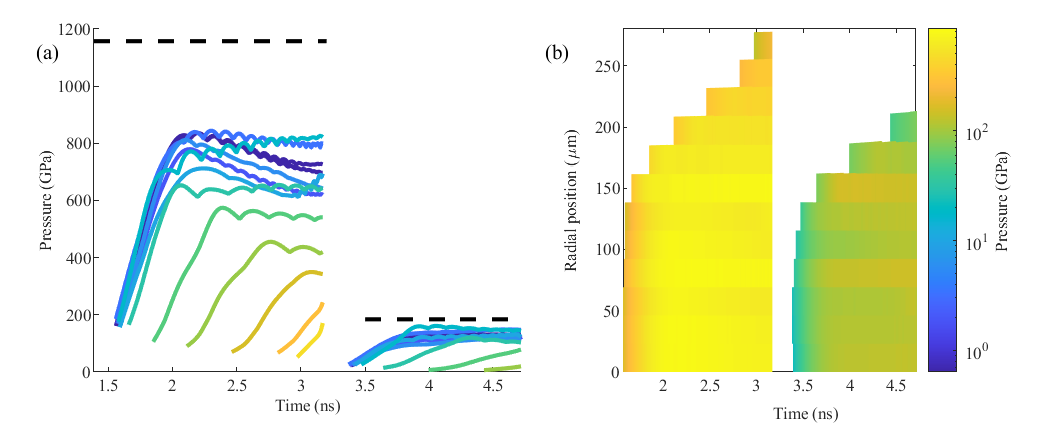
\includegraphics[width=1\textwidth]{figures/Experiment/H2DPressure.eps}% Here is how to import EPS art
\caption{\label{fig:H2DPressure} Plots showing the shock pressure in the simulation displayed in Figure \ref{fig:H2DPlot} as a function of both time and radial position. In (a), the different lines represent the different radial positions, with the colour transitioning from dark blue through to yellow (i.e. up the colour bar in Figure \ref{fig:H2DPlot}) as the radius moves further away from the center of the target. It can be seen here that the pressure is relatively uniform over the central regions, but drops off towards the edge. The dashed line represents the average shock pressure obtained in both materials in the 1D simulation. It is clear that this is significantly higher, but the difference appears to depend on simulation parameters (such as resolution) and was not observed in the other 2D codes. (b) represents the same data, but here the pressure is represnted by the colour on the 2D plot of position vs time. On both plots, the shock front pressure is only recorded when the shock front can be automatically identified in the simulation, and thus there are blank regions when the shock crosses material interfaces and the shock front cannot be clearly identified.}
\end{figure}

\begin{figure}[hbt!]
\centering
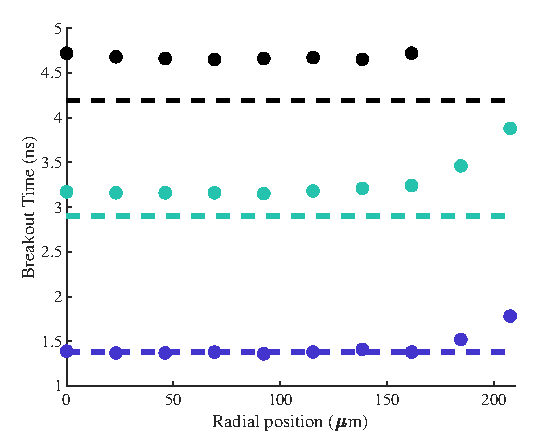
\includegraphics[width=0.6\textwidth]{figures/Experiment/H2DTiming.eps}% Here is how to import EPS art
\caption{\label{fig:H2DTiming} Shock breakout times from the gold (blue points), quartz (teal points) and foam (black points) as a function of radial position in the target. It can be seen that the breakout time is roughly steady over a radius of 150 \unit{\micro\meter}, and then increases towards the edge of the laser pulse. The dashed lines represent the breakout times obtained from the 1D Hyades simulation. While there is good agreement for the gold breakout, the 2D simulation returns a later breakout from the quartz and the foam, suggesting a slower and weaker shock. This is not observed in the other 2D simulations.  }
\end{figure}

Both Figure \ref{fig:H2DPressure} (a) and Figure \ref{fig:H2DTiming} also compare these results to the 1D Hyades simulation shown in Figure \ref{fig:PreExpHydro}. It can be seen that the timing agreement is reasonably close, but there is a small increase in the shock transit time in both the quartz and the foam. This increase in transit time is due to a decreased shock velocity, which in turn indicates a lower shock pressure as seen in Figure \ref{fig:H2DPressure}. While the change in shock transit is relatively small, the corresponding impact on the pressure is relatively significant. Interestingly, as can be seen in the post-experiment simulations, such an effect was not observed to the same extent in the simulations performed in other 2D codes. This effect (particularly the pressure) was found to vary with the resolution of the simulations, suggesting it had not fully converged; unfortunately it was not possible (due to persistent issues with mesh tangling and crashing) to increase the resolution of the simulation to a point where the results converged. As such, while the h2D simulation was useful for confirming the shock planarity and expected behaviour in 2D, it was decided that the results should not be relied on for the precise shock timings/pressures, and the other codes (such as Multi and FLASH) were used for the post-experiment 2D simulations.


%were also performed in a variety of codes, to check that the shock was relatively consistent across the shock diameter. Simulations were performed in h2D (the 2D version of Hyades) which showed that the shock behaviour was largely similar to that seen in Hyades. The shock was planar over most of the 400\unit{\micro\meter} imaged region, and the transit time was only slightly reduced compared to the 1D simulations. Piotr R\k{a}czka also performed a 2D Flash simulation which included the target step (as h2D was a lagrangian code, issues with mesh tangling prevented such a simulation from being performed) and showed that this did not significantly affect the shock propagation.

\section{Conducting the experiment}

The experiment was performed over a five and a half week period. Roughly two and a half weeks of this were setup, with a further three weeks of experimental shots. A series of images showing the experimental setup can be seen in Appendix \ref{app:experimentphotos}.

Throughout the run a number of changes were required from the original setup and experimental plan. These are outlined and explained in the following sections.

\subsection{Changes from planned target} \label{Target issues}
The actual targets that were delivered for the experiment differed slightly from the planned targets. This was due to challenges in fabricating the targets, as well as one of the suppliers failing to deliver a shipment of quartz (which also limited the number of available targets).
\begin{itemize}
    \item \textbf{Different target dimensions}: the delivered quartz was thicker than expected, which led to the quartz layer in each target being $\sim$ 50 \unit{\micro\meter} thick (rather than the planned 40 \unit{\micro\meter}). The foam thickness also varied, and was frequently significantly larger than the planned 40 \unit{\micro\meter}.
    \item \textbf{Fewer targets with an AR coating}: the reduced quantity of quartz meant that some targets did not have the planned anti-reflection coating. Fortunately, this did not seem to have a significant effect.
    \item \textbf{Delamination in some targets}: in a small number of early targets, the ablator/gold delaminated from the quartz, and had to be glued back on. The glue layer prevented an accurate timing measurement in the quartz and meant that the target could not be used for impedance matching; however, they were shot as test/setup targets. These later became important in understanding some features of the results (see Section \ref{Weak quartz shock}).
\end{itemize}

\subsection{Poor VISAR illumination and subsequent changes to optical setup}

Once setup was complete and shots started, it became apparent that the probe laser was only illuminating a small section of the imaged region. This prevented sufficient VISAR data from being collected. This was due to the fact that the probe laser travelled through the optical relay before reaching the target, which demagnified it and brought the laser to focus at the target position, as seen in Figure \ref{fig:Full experiment schematic}. 

An initial solution was to place a 700 \unit{\milli\meter} focal length lens between the laser and the VISAR beamsplitter; this would mean the laser was not collimated when entering the relay, and so would not be perfectly focussed by the objective lens. This did not sufficiently improve the problem. As such, a modified setup was designed which would solve the problem while requiring minimal changes to the optical relay (which could not be realigned due to time constraints). In the new setup, the first mirror after the objective lens was replaced with a beamsplitter, and the probe laser was injected through this beamsplitter rather than after the VISARs. This meant the probe laser bypassed the relay, and only the objective lens was shared. A lens was placed in the probe laser beampath prior to this beamsplitter to form a lens pair with the objective lens; this meant that the probe laser would be collimated by the objective lens, and thus collimated when it reached the target \footnote{While this was initially the case, extra mirrors were later added to the setup to give additional control over the probe laser position. Spatial constraints meant these mirrors had to be added between the lenses, which increased the P1-L1 distance from the intended 550mm to 875mm. This meant that the beam was no longer perfectly collimated. However, burn paper tests showed that the spot size at the target position was still sufficient, and the illumination remained uniform. Simulation of this setup with the ray tracing code suggested the spot size was around 1 mm in diameter.}. A simple schematic showing this new setup can be seen in Figure \ref{fig:Full experiment schematic with new laser setup}, with a schematic showing the spatial arrangement shown in Figure \ref{fig:Full setup}. A scale 3D CAD model and engineering drawings with measurements of this setup are provided in Appendix \ref{app:experimentphotos}.

\begin{figure}
\begin{centering}
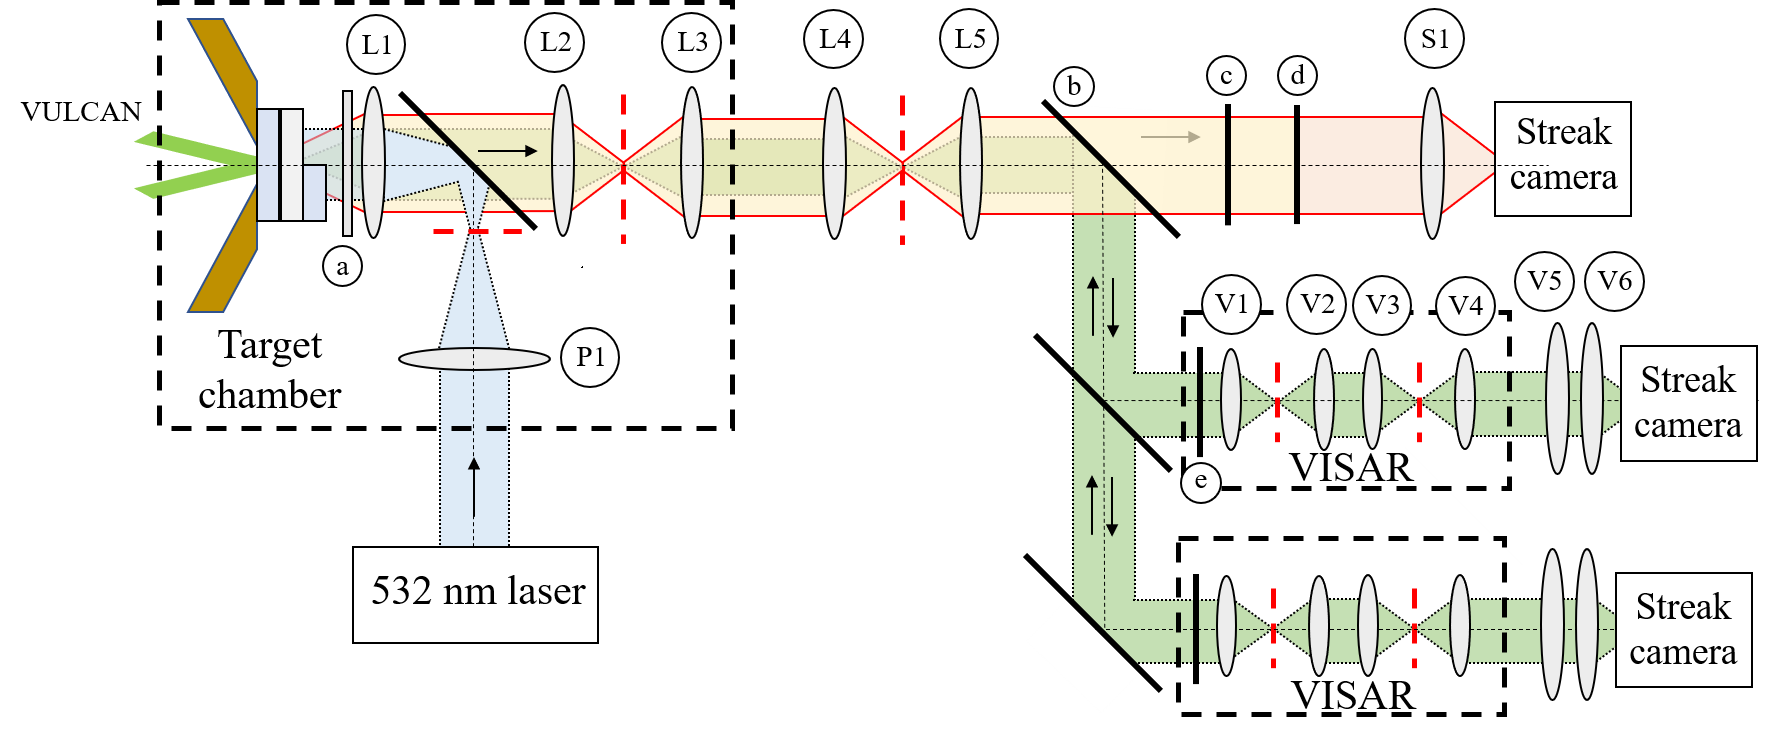
\includegraphics[width=1.0\textwidth]{figures/Experiment/Full experiment schematic new laser injection.png}% Here is how to import EPS art
\caption{\label{fig:Full experiment schematic with new laser setup} The full schematic, with the new probe laser injection. The probe laser is displayed in blue to differentiate the beampath from the reflected probe light shown in green, but both have the same 532 nm frequency. The labels are unchanged from Figure \ref{fig:Full experiment schematic}, except for a new 400 mm lens P1. This forms a lens pair with the objective lens L1; the beam passes through P1 and is focussed at the focal point of L1, so that L1 collimates the beam before it reaches the target. The incoming laser is then scattered from the target, and the objective lens is thus still considered to be collimating the reflected light. The only other changes from the original setup are the addition of a beamsplitter between L1 and L2 (replacing a mirror in the previous setup), and the replacement of the beamsplitter prior to the bottom VISAR with a mirror.}
\end{centering}
\end{figure}

\begin{figure}
\begin{centering}
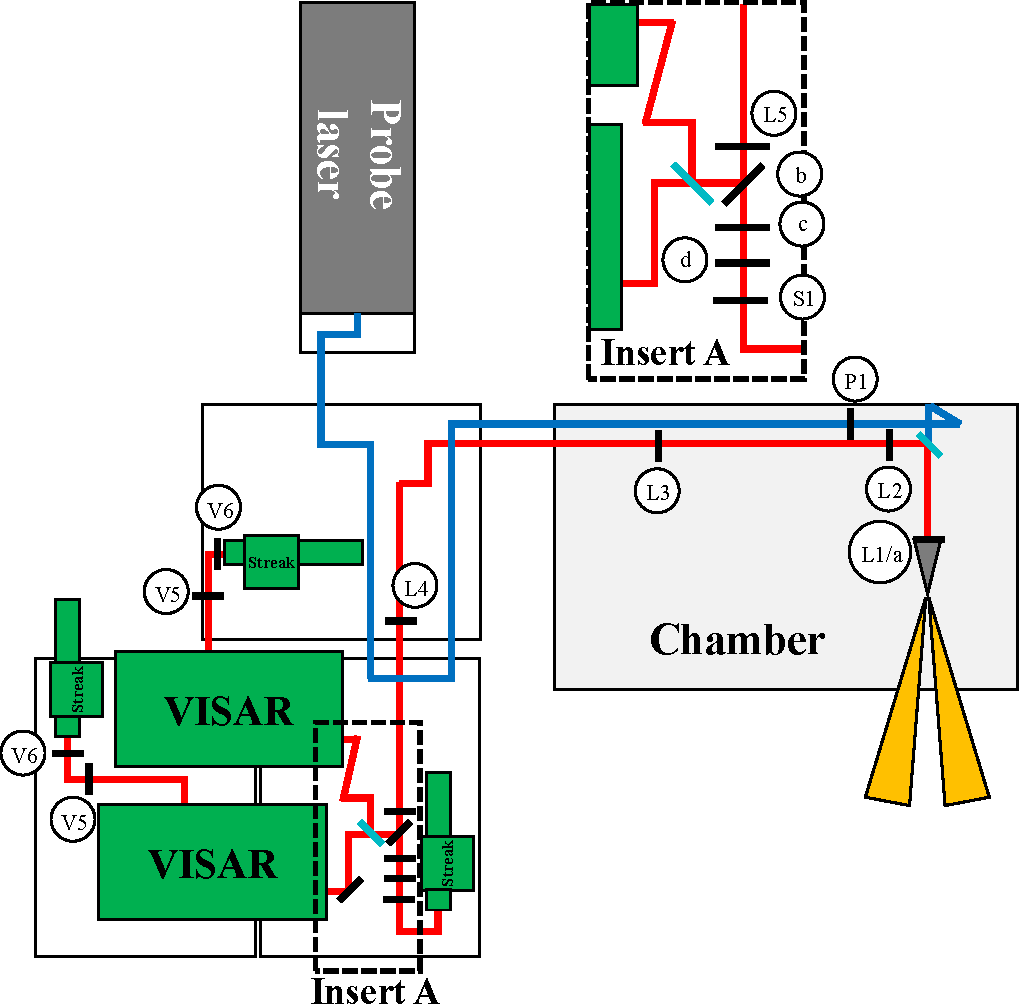
\includegraphics[width=0.8\textwidth]{figures/Experiment/FinalSetup.pdf}% Here is how to import EPS art
\caption{\label{fig:Full setup} The updated spatial arrangement. The labels are as in previous figures. The main changes are the new beampath route for the probe laser, which leads to a beamsplitter between L1 and L2 (previously a mirror), and the removal of the beamsplitter before the second VISAR (replaced with a mirror).}
\end{centering}
\end{figure}

This setup significantly improved the illumination, as shown in Figure \ref{fig:VISAR before and after}. The downside of this approach was that the beamsplitter in the relay would reduce the intensity of the captured emission (both the VISAR signal and the self-emission) by half (although the second VISAR beamsplitter could be replaced with a mirror, which compensated for the signal loss on one of the VISARs). This was a necessary sacrifice though, as without this change the illumination was not sufficient for the VISAR to be used.

\begin{figure}
\begin{centering}
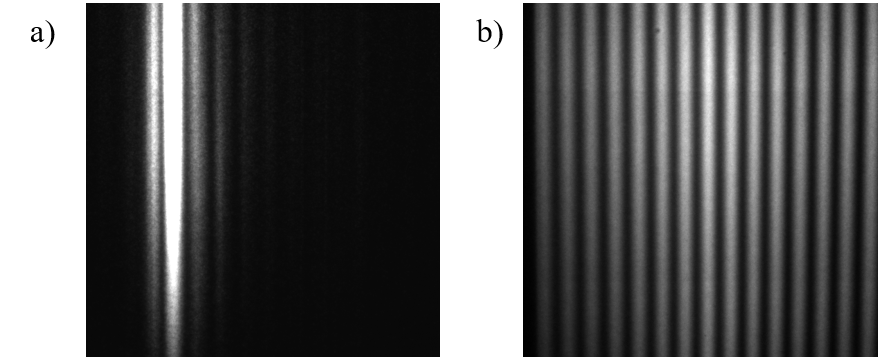
\includegraphics[width=0.8\textwidth]{figures/Experiment/VISAR before and after.png}% Here is how to import EPS art
\caption{\label{fig:VISAR before and after} Images taken in focus mode on the VISAR streak camera from a piece of quartz a) using the original setup and b) using the updated setup. The quartz sample is stationary, and the camera used in focus mode so the signal at a single time across two spatial dimensions is recorded; uniform fringes are expected across the whole image. It is clear that in (a) only part of the sample is well-illuminated, whereas the new setup well illuminates the full imaged region. The signal strength was also better using the new setup; (a) is only brighter due to different filtering.}
\end{centering}
\end{figure}

\subsection{Later than expected shock breakout times}

It was noted mid-experimental run that the shock breakout times being measured for a given intensity were significantly longer than those predicted by simulations. This meant that the VULCAN drive beam was frequently ending prior to shock breakout - contrary to the experimental plan, where the drive beam would be kept on until shock breakout to ensure a sustained shock. Additional simulations were therefore performed mid-run to determine the expected impact of the drive laser pulse ending before shock breakout time. It was found that in fact this did not lead to substantial differences in shock behaviour, and thus this was not a major cause for concern.

There was also concern that this could be due to a lower than expected laser intensity. However, the pulse time and pulse energy were directly measured for each shot using the diagnostics, and the laser spot diameter could easily be estimated from the pinhole image (the complete post-experiment analysis of this is given in Section \ref{Other diagnostic analysis}). This suggested that the intensity was as expected, and not responsible for the issue.

\subsection{Signal strength issues}

Throughout the experiment, both diagnostics suffered from a lack of signal strength. Some of this could be explained by the streak cameras. Three were used in this experiment; two high dynamic range Hamamatsu C7700 cameras were used for the VISARs, while a Hamamatsu C5680 was used for the streaked optical pyrometer. The older C5680 was expected to be less sensitive, and this was used for the SOP accordingly (as the VISAR was the more important diagnostic). This camera struggled for signal throughout. One of the VISARs also consistently recorded low signals compared to the other; it was later realised that this camera had an S1 streak tube as opposed to the S20 used in the other. The S1 tube (which was also present in the SOP streak) is around two orders of magnitude less sensitive to 532 \unit{\nano\meter} light.

The signal strength for both VISARs was also heavily influence by the probe laser. This laser was relatively high power, and significant ND filters were needed to prevent it damaging the optics in the optical chain. However, the long optical relay likely resulted in some decrease in signal strength. There were also significant operational issues with the probe laser. It frequently did not seed, resulting in the pulse being significantly weaker, and being emitted at a different time. This would occur on shots, where the low strength and change in time (relative to the VULCAN pulse) would prevent useful data from being collected. After attempting a number of fixes, the facility staff eventually replaced the seed laser within the unit with one from a different laser. This improved the situation and allowed the experiment to continue, but the timing and pulse intensity continued to vary drastically from shot to shot.

\section{Conclusion}
An overview of the experiment has been presented, along with an explanation of the diagnostics that will be used to make the measurements. The preparation for the experiment was discussed, including how the optical setup and experimental configuration was designed, and the simulations performed to assist with design of the targets. Finally, challenges that arose during the actual experiment were considered, along with the changes that were made to allow good data to be collected. The analysis of this data and the results will be discussed in the next chapter.

